\chapter{Contexto da pesquisa}

% \textcolor{red}{contexto dos projetos, desde o início, inserção dos projetos, o projeto que estou inserida (frequência), foi feita a análise da arquitetura, mas não teve a etapa da coleta. nesse caso, foi dado u passo atrás, entrou em contato com outro grupo do nees, do sistema alerta preventivo, dados não são públicos, não serão divulgados, mas o instrumento e estrutura estão nesse anexo}



No estágio inicial deste trabalho de conclusão de curso, a abordagem consistia na análise da arquitetura do sistema, fornecida pelo NEES, juntamente com uma revisão da literatura nacional e internacional sobre sistemas de coleta de frequência e algoritmos de reconhecimento de padrões baseados em machine learning. A expectativa era que os dados adquiridos pudessem ser prontamente aplicados à arquitetura futura do Sistema Presença do TED 11476. No entanto, devido à indisponibilidade dos dados desse TED específico, foi necessário um redirecionamento metodológico. Em contato com o TED 10974, responsável pelo Sistema Alerta Preventivo (SAP), foi possível obter acesso a dados não públicos do SAP. Esses dados, embora não sejam divulgados publicamente, foram fundamentais para a análise proposta, utilizando o instrumento e a estrutura fornecidos no Anexo 1, em substituição aos dados originais não obtidos.

A pesquisa teve início com a intenção de identificar padrões na base de dados proveniente do sistema de frequência do TED 11476, a qual almeja reformular o atual Sistema Presença, responsável por coletar a frequência escolar de estudantes do ensino básico vinculados ao programa Bolsa Família no Brasil \cite{BolsaFamilia}. Foi apresentada a futura arquitetura da base de dados do sistema, bem como o modelo entidade-relacionamento da coleta de frequência e como os professores teriam suas respectivas conexões. Contudo, pelo teste piloto marcado para acontecer em setembro não ter coletado dados de frequência de estudantes, e por não ter sido possível conseguir uma base de dados legada do Sistema Presença vigente, a etapa do estudo de dados do TED 11476 não pôde ser concretizada conforme inicialmente previsto. Na tentativa de se realizar uma base de dados sintética, foi solicitada a base do TED 10974, esperando compreender diferentes motivações de evasão escolar a serem replicadas na arquitetura disponibilizada. Porém, embora tenha implicado em uma regressão no processo planejado, foi optado pelo foco nos dados disponibilizados pelo TED 10974, utilizando os algoritmos estudados anteriormente para aplicação nessa base.

Assim, o foco metodológico da pesquisa passou a envolver a análise da arquitetura do SAP, utilizando os dados disponíveis. Este passo foi considerado necessário para avançar no entendimento dos fatores de risco de evasão escolar. Este ajuste metodológico permitiu uma continuidade efetiva na análise do contexto do Sistema Alerta Preventivo, oferecendo insights valiosos para a compreensão dos fatores relacionados à evasão escolar no contexto específico do projeto.

Tanto o questionário das perguntas relacionadas a evasão quanto as perguntas sociodemográficas estão disponibilizadas neste trabalho como Anexo 1.


\section{Questionário Sistema Alerta Preventivo}
\label{cap:analises-sap}

% Os dados disponibilizados foram organizados de acordo com os relacionamentos dos estudantes com diversos fatores chamados de dimensão de risco estudante-escola (E-ESC), Estudante - profissionais da escola (e-prof), Estudante-familia(e-fam), estudante-comunidade (E-COM) e também com seus semelhantes estudante-estudante (e-est).
% Dos 17 mil respondentes das 35 perguntas e dentro de cada tipo de relacionamento organizou-se os fatores de risco dentro de cada relacionamento com tres perguntas em cada um. Condições Materiais da Escola (e-esc1), condicões Materias do(a) estudante (E-ESC2),  Inflexibilidade
% Pedagógica
% (E-PROF1), Qualidade
% Pedagógica
% (E-PROF2), Suporte Familiar
% (E-FAM1), Gravidez/parentalidade/
% atividades de cuidado
% (E-FAM2), Medidas
% socioeducativas e
% contextos de
% violência(E-COM1), Acessibilidade e
% frequência escolar
% (E-COM2), Distanciamento
% escola –
% comunidade
% (E-COM3), Significados da
% Escolarização/
% Engajamento
% (E-EST1), Aspectos
% Emocionais e
% Afetivos(E-EST2), Reprovações e
% distorção idade –
% série. (E-EST3).

O banco de dados disponibilizado pelo NEES, referente ao SAP, foi realizado com 17.110 estudantes de forma presencial em dezembro de 2022. O banco compilou e categorizou dados cruciais para compreender as multifacetadas dimensões de risco de evasão, que podem ser afetados a partir da relação entre estudantes e seus ambientes escolares, domésticos e comunitários, bem como suas interações entre pares. Este arcabouço de informação, constituído por respostas de alunos do primeiro ao nono ano do ensino fundamental de 308 escolas diferentes, a 36 questões distintas, constitui uma base sólida para a investigação das causas subjacentes à evasão escolar. Cada pergunta era respondida por meio de uma escala de Likert, onde as respostas eram valores inteiros entre 1 (Discordo Totalmente) e 7 (Concordo Totalmente), sendo que os estudantes podiam optar por não responder às perguntas, atribuindo valor 0 à pergunta. As perguntas foram separadas em grupos de análise de fatores de risco, e dois ou três fatores eram agrupados em uma única dimensão analisada. Esta organização é apresentada na Tabela \ref{tab:questionario}.

Dentro deste contexto, a dimensão \textbf{Estudante-Escola (E-ESC)} lança luz sobre as condições materiais das instituições de ensino. Este aspecto envolve não apenas a infraestrutura física mas também recursos didáticos essenciais para um ambiente de aprendizagem eficaz. Além disso, examina-se a realidade material dos próprios estudantes, percebendo como a escassez de recursos pode influenciar negativamente a permanência na escola.

Por outro lado, a relação \textbf{Estudante-Profissionais da Escola (E-PROF)} aborda a rigidez e a qualidade pedagógica. Aqui, a inflexibilidade pedagógica surge como um fator de risco potencial, pois pode desencorajar os estudantes cujas necessidades educacionais variam. Em contrapartida, a qualidade do ensino detém uma influência crítica, já que a excelência pedagógica e a atenção individualizada podem diminuir as chances de abandono escolar.

No que tange à dimensão \textbf{Estudante-Família (E-FAM)}, o suporte familiar é analisado como um alicerce essencial para a continuidade educacional. Desafios como gravidez na adolescência, parentalidade precoce e obrigações de cuidado podem desviar a atenção e os recursos dos estudantes da educação para responsabilidades familiares, aumentando o risco de evasão.

A relação \textbf{Estudante-Comunidade (E-COM)} explora como medidas socioeducativas e a prevalência de violência no entorno podem criar barreiras ao acesso e à frequência escolar, além de como a desconexão entre a escola e a comunidade pode acentuar a sensação de isolamento dos estudantes, diminuindo a valorização da educação em seus contextos de vida.

Finalmente, na esfera \textbf{Estudante-Estudante (E-EST)}, observa-se o impacto do engajamento escolar e os significados atribuídos à escolarização, bem como as interações emocionais e afetivas entre os estudantes, e como repetências e defasagens idade-série podem desmotivar os alunos e conduzi-los ao abandono do sistema educacional.

    
\begin{longtable}{|@{}>{\centering\arraybackslash}p{0.25\textwidth}| >{\centering\arraybackslash\scriptsize}p{\dimexpr 0.23\textwidth - 24pt\relax}| >{\centering\arraybackslash}p{0.12\textwidth}| >{\raggedright\arraybackslash\scriptsize}p{0.35\textwidth}@{}|}
\caption{Perguntas do questionário associadas a fatores e dimensões}
\label{tab:questionario}

\hline
\textbf{Dimensão de Risco} &
  \textbf{Fatores de Risco} &
  \textbf{\begin{tabular}[c]{@{}c@{}}Código da\\ Pergunta\end{tabular}} &
  \multicolumn{1}{c|}{\textbf{Itens}} \\ \hline
\endhead
\multirow{6}{*}{\textbf{\begin{tabular}[c]{@{}c@{}}Estudante –\\ Escola (E-ESC)\end{tabular}}} &
  \multirow{3}{*}{\begin{tabular}[c]{@{}c@{}}Condições\\ Materiais da Escola\\ (E-ESC1)\end{tabular}} &
  Q3 &
  \begin{tabular}[c]{@{}l@{}}A alimentação oferecida na escola me faz\\ pensar em não ir para ela.\end{tabular} \\ \cline{3-4} 
 &
   &
  Q4 &
  \begin{tabular}[c]{@{}l@{}}Pensei em me afastar da escola por não ter\\ equipamentos adequados para lidar com as\\ condições do clima (ventilador, aquecedor,\\ ar condicionado).\end{tabular} \\ \cline{3-4} 
 &
   &
  Q23 &
  \begin{tabular}[c]{@{}l@{}}Não poder usar a internet na escola é algo\\ que me faz querer me afastar.\end{tabular} \\ \cline{2-4} 
 &
  \multirow{3}{*}{\begin{tabular}[c]{@{}c@{}}Condições\\ Materiais do(a)\\ Estudante (E-ESC2)\end{tabular}} &
  Q9 &
  \begin{tabular}[c]{@{}l@{}}Pensei em sair da escola porque não tenho\\ um bom espaço em casa para me\\ concentrar nos estudos.\end{tabular} \\ \cline{3-4} 
 &
   &
  Q28 &
  \begin{tabular}[c]{@{}l@{}}Possuo o material escolar adequado para\\ acompanhar as aulas (lápis, caderno, etc.).\end{tabular} \\ \cline{3-4} 
 &
   &
  Q36 &
  \begin{tabular}[c]{@{}l@{}}Não possuo o fardamento escolar\\ adequado.\end{tabular} \\ \hline
\multirow{6}{*}{\textbf{\begin{tabular}[c]{@{}c@{}}Estudante –\\ Profissionais da\\ Escola (E-PROF)\end{tabular}}} &
  \multirow{3}{*}{\begin{tabular}[c]{@{}c@{}}Inflexibilidade\\ Pedagógica\\ (E-PROF1)\end{tabular}} &
  Q13 &
  \begin{tabular}[c]{@{}l@{}}Pensei em me afastar da escola pela\\ quantidade de regras que ela tem.\end{tabular} \\ \cline{3-4} 
 &
   &
  Q18 &
  \begin{tabular}[c]{@{}l@{}}Penso em deixar a escola porque ela não\\ me permite fazer atividades como música,\\ dança, teatro, desenho.\end{tabular} \\ \cline{3-4} 
 &
   &
  Q22 &
  \begin{tabular}[c]{@{}l@{}}Pensei em abandonar a escola por não\\ poder praticar os esportes que eu queria.\end{tabular} \\ \cline{2-4} 
 &
  \multirow{3}{*}{\begin{tabular}[c]{@{}c@{}}Qualidade\\ Pedagógica\\ (E-PROF2)\end{tabular}} &
  Q12 &
  \begin{tabular}[c]{@{}l@{}}Pensei em abandonar a escola pois os (as)\\ professores (as) faltam muito.\end{tabular} \\ \cline{3-4} 
 &
   &
  Q19 &
  \begin{tabular}[c]{@{}l@{}}Pensei em abandonar a escola porque as\\ salas têm mais estudantes do que os\\ professores conseguem dar atenção.\end{tabular} \\ \cline{3-4} 
 &
   &
  Q20 &
  \begin{tabular}[c]{@{}l@{}}Pensei em abandonar a escola pois as aulas\\ são repetitivas e cansativas.\end{tabular} \\ \hline
\multirow{6}{*}{\textbf{\begin{tabular}[c]{@{}c@{}}Estudante –\\ Família (E-FAM)\end{tabular}}} &
  \multirow{3}{*}{\begin{tabular}[c]{@{}c@{}}Suporte Familiar\\ (E-FAM1)\end{tabular}} &
  \multicolumn{1}{c|}{Q16} &
  \begin{tabular}[c]{@{}l@{}}Alguém da minha família já sugeriu que eu\\ deixasse a escola.\end{tabular} \\ \cline{3-4} 
 &
   &
  \multicolumn{1}{c|}{Q30} &
  \begin{tabular}[c]{@{}l@{}}Meus pais/responsáveis não podem vir à\\ escola quando são chamados.\end{tabular} \\ \cline{3-4} 
 &
   &
  \multicolumn{1}{c|}{Q32} &
  \begin{tabular}[c]{@{}l@{}}Minha mãe, ou a pessoa que cuida de mim,\\ não terminou a escola.\end{tabular} \\ \cline{2-4} 
 &
  \multirow{3}{*}{\begin{tabular}[c]{@{}c@{}}Gravidez/parentalidade/\\ atividades de cuidado\\ (E-FAM2)\end{tabular}} &
  \multicolumn{1}{c|}{Q15} &
  \begin{tabular}[c]{@{}l@{}}Já faltei à escola ou deixei de fazer lição\\ de casa por ter que ajudar em atividades\\ de casa (cozinhar, limpar, cuidar de\\ irmãos etc).\end{tabular} \\ \cline{3-4} 
 &
   &
  \multicolumn{1}{c|}{Q21} &
  \begin{tabular}[c]{@{}l@{}}Já pensei em abandonar a escola por ter\\ tido e/ou ter um problema de saúde na\\ família.\end{tabular} \\ \cline{3-4} 
 &
   &
  \multicolumn{1}{c|}{Q31} &
  \begin{tabular}[c]{@{}l@{}}Já aconteceu de eu não poder continuar na\\ escola por causa de uma gravidez, seja\\ minha ou da minha parceira.\end{tabular} \\ \hline

  \multirow{9}{*}{\textbf{\begin{tabular}[c]{@{}c@{}}Estudante –\\ Comunidade\\ (E-COM)\end{tabular}}} &
  \multirow{3}{*}{\begin{tabular}[c]{@{}c@{}}Medidas\\ socioeducativas e\\ contextos de\\ violência(E-COM1)\end{tabular}} &
  Q29 &
  \begin{tabular}[c]{@{}l@{}}Meus colegas frequentemente abusam de\\ álcool ou drogas.\end{tabular} \\ \cline{3-4} 
 &
   &
  Q33 &
  \begin{tabular}[c]{@{}l@{}}Já tive/tenho contato com o Conselho\\ Tutelar.\end{tabular} \\ \cline{3-4} 
 &
   &
  Q34 &
  \begin{tabular}[c]{@{}l@{}}É comum que na minha escola estudantes\\ enfrentem problemas com a justiça.\end{tabular} \\ \cline{2-4} 
 &
  \multirow{3}{*}{\begin{tabular}[c]{@{}c@{}}Acessibilidade e\\ frequência escolar\\ (E-COM2)\end{tabular}} &
  Q8 &
  \begin{tabular}[c]{@{}l@{}}Já pensei em deixar a escola porque não\\ tenho aulas sobre a história ou questões\\ importantes da minha comunidade ou\\ cidade.\end{tabular} \\ \cline{3-4} 
 &
   &
  Q11 &
  \begin{tabular}[c]{@{}l@{}}Já pensei em deixar a escola porque ela\\ não respeita a religião que eu pratico.\end{tabular} \\ \cline{3-4} 
 &
   &
  Q14 &
  \begin{tabular}[c]{@{}l@{}}Já pensei em deixar a escola porque com\\ frequência ela é alvo de violência\\ (vandalismo, assaltos, pichações, toque de\\ recolher e etc).\end{tabular} \\ \cline{2-4} 
 &
  \multirow{3}{*}{\begin{tabular}[c]{@{}c@{}}Distanciamento\\ escola –\\ comunidade\\ (E-COM3)\end{tabular}} &
  Q7 &
  \begin{tabular}[c]{@{}l@{}}Já considerei abandonar a escola por ter\\ tido e/ou ter um problema de saúde.\end{tabular} \\ \cline{3-4} 
 &
   &
  Q17 &
  \begin{tabular}[c]{@{}l@{}}Pensei em abandonar a escola porque não\\ tenho dinheiro suficiente para vir ou\\ porque o caminho até aqui é muito difícil.\end{tabular} \\ \cline{3-4} 
 &
   &
  Q25 &
  Falto às aulas mais do que é permitido. \\ \hline
  
\multirow{9}{*}{\textbf{\begin{tabular}[c]{@{}c@{}}Estudante –\\ Estudante\\ (E-EST)\end{tabular}}} &
  \multicolumn{1}{l|}{\multirow{3}{*}{\begin{tabular}[c]{@{}l@{}}Significados da\\ Escolarização/\\ Engajamento\\ (E-EST1)\end{tabular}}} &
  Q5 &
  \begin{tabular}[c]{@{}l@{}}Já pensei em abandonar a escola porque\\ não vejo como ela vai me ajudar a mudar\\ minha vida para melhor.\end{tabular} \\ \cline{3-4} 
 &
  \multicolumn{1}{l|}{} &
  Q6 &
  \begin{tabular}[c]{@{}l@{}}Pensei em deixar a escola pois ela não\\ trata dos assuntos atuais.\end{tabular} \\ \cline{3-4} 
 &
  \multicolumn{1}{l|}{} &
  Q10 &
  \begin{tabular}[c]{@{}l@{}}Já pensei em abandonar a escola pois ela\\ não me prepara para os empregos que\\ quero ter no futuro.\end{tabular} \\ \cline{2-4} 
 &
 
  \multicolumn{1}{l|}{\multirow{3}{*}{\begin{tabular}[c]{@{}l@{}}Aspectos\\ Emocionais e\\ Afetivos(E-EST2)\end{tabular}}} &
  Q1 &
  \begin{tabular}[c]{@{}l@{}}Às vezes, me sinto triste ou deprimido(a),\\ e isso me faz pensar em deixar a escola.\end{tabular} \\ \cline{3-4} 
 &
  \multicolumn{1}{l|}{} &
  Q2 &
  \begin{tabular}[c]{@{}l@{}}Sinto que sou incapaz de concluir meus\\ estudos e por isso penso em abandonar a\\ escola.\end{tabular} \\ \cline{3-4} 
 &
  \multicolumn{1}{l|}{} &
  Q24 &
  \begin{tabular}[c]{@{}l@{}}Já pensei em deixar a escola porque\\ meus/minhas colegas não me tratam bem.\end{tabular} \\ \cline{2-4} 
 &
  \multicolumn{1}{l|}{\multirow{3}{*}{\begin{tabular}[c]{@{}l@{}}Reprovações e\\ distorção idade –\\ série. (E-EST3)\end{tabular}}} &
  Q26 &
  \begin{tabular}[c]{@{}l@{}}Acredito que tenho mais dificuldade de\\ acompanhar as aulas do que os outros\\ colegas.\end{tabular} \\ \cline{3-4} 
 &
  \multicolumn{1}{l|}{} &
  Q27 &
  \begin{tabular}[c]{@{}l@{}}Minhas notas em Poutuguês e/ou\\ Matemática estão abaixo da média.\end{tabular} \\ \cline{3-4} 
 &
  \multicolumn{1}{l|}{} &
  Q35 &
  \begin{tabular}[c]{@{}l@{}}Não estou na série que deveria estar para\\ a minha idade.\end{tabular} \\ \hline
\end{longtable}
\fonte{NEES - TED 10479 (2022)}

% \begin{table}[ht]
% \centering
% \resizebox{\textwidth}{!}{%
% \begin{tabular}{|c|c|c|l|}
% \hline
% \textbf{Dimensão de Risco} &
%   \textbf{Fatores de Risco} &
%   \textbf{\begin{tabular}[c]{@{}c@{}}Código da\\ Pergunta\end{tabular}} &
%   \multicolumn{1}{c|}{\textbf{Itens}} \\ \hline
% \multirow{6}{*}{\textbf{\begin{tabular}[c]{@{}c@{}}Estudante –\\ Escola (E-ESC)\end{tabular}}} &
%   \multirow{3}{*}{\begin{tabular}[c]{@{}c@{}}Condições\\ Materiais da Escola\\ (E-ESC1)\end{tabular}} &
%   Q3 &
%   \begin{tabular}[c]{@{}l@{}}A alimentação oferecida na escola me faz\\ pensar em não ir para ela.\end{tabular} \\ \cline{3-4} 
%  &
%    &
%   Q4 &
%   \begin{tabular}[c]{@{}l@{}}Pensei em me afastar da escola por não ter\\ equipamentos adequados para lidar com as\\ condições do clima (ventilador, aquecedor,\\ ar condicionado).\end{tabular} \\ \cline{3-4} 
%  &
%    &
%   Q23 &
%   \begin{tabular}[c]{@{}l@{}}Não poder usar internet na escola é algo\\ que me faz querer me afastar.\end{tabular} \\ \cline{2-4} 
%  &
%   \multirow{3}{*}{\begin{tabular}[c]{@{}c@{}}Condições\\ Materiais do(a)\\ Estudante (E-ESC2)\end{tabular}} &
%   Q9 &
%   \begin{tabular}[c]{@{}l@{}}Pensei em sair da escola porque não tenho\\ um bom espaço em casa para me\\ concentrar nos estudos.\end{tabular} \\ \cline{3-4} 
%  &
%    &
%   Q28 &
%   \begin{tabular}[c]{@{}l@{}}Possuo o material escolar adequado para\\ acompanhar as aulas (lápis, caderno, etc.).\end{tabular} \\ \cline{3-4} 
%  &
%    &
%   Q36 &
%   \begin{tabular}[c]{@{}l@{}}Não possuo o fardamento escolar\\ adequado.\end{tabular} \\ \hline
% \multirow{6}{*}{\textbf{\begin{tabular}[c]{@{}c@{}}Estudante –\\ Profissionais da\\ Escola (E-PROF)\end{tabular}}} &
%   \multirow{3}{*}{\begin{tabular}[c]{@{}c@{}}Inflexibilidade\\ Pedagógica\\ (E-PROF1)\end{tabular}} &
%   Q13 &
%   \begin{tabular}[c]{@{}l@{}}Pensei em me afastar da escola pela\\ quantidade de regras que ela tem.\end{tabular} \\ \cline{3-4} 
%  &
%    &
%   Q18 &
%   \begin{tabular}[c]{@{}l@{}}Penso em deixar a escola porque ela não\\ me permite fazer atividades como música,\\ dança, teatro, desenho.\end{tabular} \\ \cline{3-4} 
%  &
%    &
%   Q22 &
%   \begin{tabular}[c]{@{}l@{}}Pensei em abandonar a escola por não\\ poder praticar os esportes que eu queria.\end{tabular} \\ \cline{2-4} 
%  &
%   \multirow{3}{*}{\begin{tabular}[c]{@{}c@{}}Qualidade\\ Pedagógica\\ (E-PROF2)\end{tabular}} &
%   Q12 &
%   \begin{tabular}[c]{@{}l@{}}Pensei em abandonar a escola pois os (as)\\ professores (as) faltam muito.\end{tabular} \\ \cline{3-4} 
%  &
%    &
%   Q19 &
%   \begin{tabular}[c]{@{}l@{}}Pensei em abandonar a escola porque as\\ salas têm mais estudantes do que os\\ professores conseguem dar atenção.\end{tabular} \\ \cline{3-4} 
%  &
%    &
%   Q20 &
%   \begin{tabular}[c]{@{}l@{}}Pensei em abandonar a escola pois as aulas\\ são repetitivas e cansativas.\end{tabular} \\ \hline
% \multirow{6}{*}{\textbf{\begin{tabular}[c]{@{}c@{}}Estudante –\\ Família (E-FAM)\end{tabular}}} &
%   \multirow{3}{*}{\begin{tabular}[c]{@{}c@{}}Suporte Familiar\\ (E-FAM1)\end{tabular}} &
%   \multicolumn{1}{c|}{Q16} &
%   \begin{tabular}[c]{@{}l@{}}Alguém da minha família já sugeriu que eu\\ deixasse a escola.\end{tabular} \\ \cline{3-4} 
%  &
%    &
%   \multicolumn{1}{c|}{Q30} &
%   \begin{tabular}[c]{@{}l@{}}Meus pais/responsáveis não podem vir à\\ escola quando são chamados.\end{tabular} \\ \cline{3-4} 
%  &
%    &
%   \multicolumn{1}{c|}{Q32} &
%   \begin{tabular}[c]{@{}l@{}}Minha mãe, ou a pessoa que cuida de mim,\\ não terminou a escola.\end{tabular} \\ \cline{2-4} 
%  &
%   \multirow{3}{*}{\begin{tabular}[c]{@{}c@{}}Gravidez/parentalidade/\\ atividades de cuidado\\ (E-FAM2)\end{tabular}} &
%   \multicolumn{1}{c|}{Q15} &
%   \begin{tabular}[c]{@{}l@{}}Já faltei à escola ou deixei de fazer lição\\ de casa por ter que ajudar em atividades\\ de casa (cozinhar, limpar, cuidar de\\ irmãos etc).\end{tabular} \\ \cline{3-4} 
%  &
%    &
%   \multicolumn{1}{c|}{Q21} &
%   \begin{tabular}[c]{@{}l@{}}Já pensei em abandonar a escola por ter\\ tido e/ou ter um problema de saúde na\\ família.\end{tabular} \\ \cline{3-4} 
%  &
%    &
%   \multicolumn{1}{c|}{Q31} &
%   \begin{tabular}[c]{@{}l@{}}Já aconteceu de eu não poder continuar na\\ escola por causa de uma gravidez, seja\\ minha ou da minha parceira.\end{tabular} \\ \hline
% \end{tabular}%
% }
% \caption{Perguntas do questionário associadas a fatores e dimensões}
% \end{table}


% \begin{table}[ht]
% \centering
% \resizebox{\textwidth}{!}{%
% \begin{tabular}{|c|c|c|l|}
% \hline
% \textbf{Dimensão de Risco} &
%   \textbf{Fatores de Risco} &
%   \multicolumn{1}{c|}{\textbf{\begin{tabular}[c]{@{}c@{}}Código da\\ Pergunta\end{tabular}}} &
%   \multicolumn{1}{c|}{\textbf{Itens}} \\ \hline
% \multirow{9}{*}{\textbf{\begin{tabular}[c]{@{}c@{}}Estudante –\\ Comunidade\\ (E-COM)\end{tabular}}} &
%   \multirow{3}{*}{\begin{tabular}[c]{@{}c@{}}Medidas\\ socioeducativas e\\ contextos de\\ violência(E-COM1)\end{tabular}} &
%   Q29 &
%   \begin{tabular}[c]{@{}l@{}}Meus colegas frequentemente abusam de\\ álcool ou drogas.\end{tabular} \\ \cline{3-4} 
%  &
%    &
%   Q33 &
%   \begin{tabular}[c]{@{}l@{}}Já tive/tenho contato com o Conselho\\ Tutelar.\end{tabular} \\ \cline{3-4} 
%  &
%    &
%   Q34 &
%   \begin{tabular}[c]{@{}l@{}}É comum que na minha escola estudantes\\ enfrentem problemas com a justiça.\end{tabular} \\ \cline{2-4} 
%  &
%   \multirow{3}{*}{\begin{tabular}[c]{@{}c@{}}Acessibilidade e\\ frequência escolar\\ (E-COM2)\end{tabular}} &
%   Q8 &
%   \begin{tabular}[c]{@{}l@{}}Já pensei em deixar a escola porque não\\ tenho aulas sobre a história ou questões\\ importantes da minha comunidade ou\\ cidade.\end{tabular} \\ \cline{3-4} 
%  &
%    &
%   Q11 &
%   \begin{tabular}[c]{@{}l@{}}Já pensei em deixar a escola porque ela\\ não respeita a religião que eu pratico.\end{tabular} \\ \cline{3-4} 
%  &
%    &
%   Q14 &
%   \begin{tabular}[c]{@{}l@{}}Já pensei em deixar a escola porque com\\ frequência ela é alvo de violência\\ (vandalismo, assaltos, pichações, toque de\\ recolher e etc).\end{tabular} \\ \cline{2-4} 
%  &
%   \multirow{3}{*}{\begin{tabular}[c]{@{}c@{}}Distanciamento\\ escola –\\ comunidade\\ (E-COM3)\end{tabular}} &
%   Q7 &
%   \begin{tabular}[c]{@{}l@{}}Já considerei abandonar a escola por ter\\ tido e/ou ter um problema de saúde.\end{tabular} \\ \cline{3-4} 
%  &
%    &
%   Q17 &
%   \begin{tabular}[c]{@{}l@{}}Pensei em abandonar a escola porque não\\ tenho dinheiro suficiente para vir ou\\ porque o caminho até aqui é muito difícil.\end{tabular} \\ \cline{3-4} 
%  &
%    &
%   Q25 &
%   Falto às aulas mais do que é permitido. \\ \hline
% \multirow{9}{*}{\textbf{\begin{tabular}[c]{@{}c@{}}Estudante –\\ Estudante\\ (E-EST)\end{tabular}}} &
%   \multicolumn{1}{l|}{\multirow{3}{*}{\begin{tabular}[c]{@{}l@{}}Significados da\\ Escolarização/\\ Engajamento\\ (E-EST1)\end{tabular}}} &
%   Q5 &
%   \begin{tabular}[c]{@{}l@{}}Já pensei em abandonar a escola porque\\ não vejo como ela vai me ajudar a mudar\\ minha vida para melhor.\end{tabular} \\ \cline{3-4} 
%  &
%   \multicolumn{1}{l|}{} &
%   Q6 &
%   \begin{tabular}[c]{@{}l@{}}Pensei em deixar a escola pois ela não\\ trata dos assuntos atuais.\end{tabular} \\ \cline{3-4} 
%  &
%   \multicolumn{1}{l|}{} &
%   Q10 &
%   \begin{tabular}[c]{@{}l@{}}Já pensei em abandonar a escola pois ela\\ não me prepara para os empregos que\\ quero ter no futuro.\end{tabular} \\ \cline{2-4} 
%  &
%   \multicolumn{1}{l|}{\multirow{3}{*}{\begin{tabular}[c]{@{}l@{}}Aspectos\\ Emocionais e\\ Afetivos(E-EST2)\end{tabular}}} &
%   Q1 &
%   \begin{tabular}[c]{@{}l@{}}Às vezes, me sinto triste ou deprimido(a),\\ e isso me faz pensar em deixar a escola.\end{tabular} \\ \cline{3-4} 
%  &
%   \multicolumn{1}{l|}{} &
%   Q2 &
%   \begin{tabular}[c]{@{}l@{}}Sinto que sou incapaz de concluir meus\\ estudos e por isso penso em abandonar a\\ escola.\end{tabular} \\ \cline{3-4} 
%  &
%   \multicolumn{1}{l|}{} &
%   Q24 &
%   \begin{tabular}[c]{@{}l@{}}Já pensei em deixar a escola porque\\ meus/minhas colegas não me tratam bem.\end{tabular} \\ \cline{2-4} 
%  &
%   \multicolumn{1}{l|}{\multirow{3}{*}{\begin{tabular}[c]{@{}l@{}}Reprovações e\\ distorção idade –\\ série. (E-EST3)\end{tabular}}} &
%   Q26 &
%   \begin{tabular}[c]{@{}l@{}}Acredito que tenho mais dificuldade de\\ acompanhar as aulas do que os outros\\ colegas.\end{tabular} \\ \cline{3-4} 
%  &
%   \multicolumn{1}{l|}{} &
%   Q27 &
%   \begin{tabular}[c]{@{}l@{}}Minhas notas em Poutuguês e/ou\\ Matemática estão abaixo da média.\end{tabular} \\ \cline{3-4} 
%  &
%   \multicolumn{1}{l|}{} &
%   Q35 &
%   \begin{tabular}[c]{@{}l@{}}Não estou na série que deveria estar para\\ a minha idade.\end{tabular} \\ \hline
% \end{tabular}%
% }
% \caption{Perguntas do questionário associadas a fatores e dimensões}
% \end{table}


%%%%%%%%%%%%%%%%%%%%%%%%%%%%%%%%%%%%%%
%%%%%%%%%%%%%%%%%%%%%%%%%%%%%%%%%%%%%%
%%%%%%%%%%%%%%%%%%%%%%%%%%%%%%%%%%%%%%
%%%%%%%%%%%%%%%%%%%%%%%%%%%%%%%%%%%%%%

\section{Análises descritivas}



Em uma visão mais ampla, observando-se a Dimensão dos Riscos, os dados permitem uma visão detalhada das percepções e experiências dos estudantes em relação a tais fatores e suas potencialidades dentro de suas escolas e comunidades, bem como em relação à sua saúde emocional e engajamento acadêmico.

A análise das respostas dos estudantes revela informações interessantes sobre a percepção que têm de sua experiência educacional, como pode ser observado na Tabela \ref{tab:estatisticas}. A dimensão ``Estus pfedante – Comunidade (E-COM)'' que inclui aspectos como o impacto da violência e problemas com a justiça, bem como questões de acessibilidade e identificação com o currículo escolar. As médias para estas dimensões (E-COMV) mostram uma pontuação de 1.677947, sugerindo uma percepção relativamente baixa dos riscos associados. Ainda assim, há uma variação considerável, como indicado pelo desvio padrão de 0.873904, que aponta para experiências distintas entre os alunos nesta dimensão.

As preocupações sobre o distanciamento entre a escola e a comunidade, assim como as dificuldades financeiras e de saúde que impactam a frequência às aulas, são também indicativas de barreiras significativas que podem influenciar a decisão dos estudantes de permanecer na escola. Questões de saúde e financeiras, especificamente, parecem ser menos mencionadas como razões para pensar em abandonar a escola, o que é ilustrado pela mediana de 1.333333, indicando que mais da metade dos estudantes classificou estas preocupações abaixo da média de risco percebido.

Quando observa-se a dimensão ``Estudante – Estudante (E-EST)'', é possível observar que os alunos têm uma visão crítica sobre o significado e relevância da educação em suas vidas. A média para essa dimensão é de 1.671151, o que indica que muitos estudantes questionam como a escola contribui para sua preparação para o futuro e refletem sobre o conteúdo do currículo em relação aos empregos desejados e às questões atuais. Isso é reforçado pela proximidade da média e da mediana, mostrando uma tendência central comum nas respostas. Os aspectos emocionais e afetivos também são uma preocupação, com questões como sentir-se triste ou deprimido e não ser bem tratado pelos colegas. %Isso aponta para a importância do ambiente escolar ser acolhedor e inclusivo para manter os estudantes engajados. A questão da reprovação e da distorção idade-série também aparece nas respostas, sinalizando que há estudantes que se sentem em desvantagem e isso pode contribuir para o desejo de deixar a escola.

Em termos de variação, as pontuações mínimas e máximas para todas as dimensões variam de 0.0 a valores próximos a 7, o que indica que há estudantes que não percebem esses fatores como um risco, enquanto outros os avaliam como bastante significativos. Essa ampla gama reflete a diversidade das experiências e percepções dos estudantes em relação à sua educação e ambiente escolar.


\begin{table}[ht]
    \centering
    \caption{Tabela de Estatísticas de Dimensões}
    \label{tab:estatisticas}
    \begin{tabular}{|c|c|c|c|c|c|}
        \hline
        \textbf{Dimensão} & \textbf{Média} & \textbf{Desvio Padrão} & \textbf{Mediana} & \textbf{Mínimo} & \textbf{Máximo} \\
        \hline
        E\_ESCV & 1.764666 & 0.958435 & 1.416667 & 0.0 & 7.000000 \\
        E\_PROFV & 1.504817 & 1.067959 & 1.000000 & 0.0 & 7.000000 \\
        E\_FAMV & 1.489781 & 0.784556 & 1.000000 & 0.0 & 6.833333 \\
        E\_COMV & 1.677947 & 0.873904 & 1.333333 & 0.0 & 7.000000 \\
        E\_ESTV & 1.671151 & 0.862080 & 1.333333 & 0.0 & 6.500000 \\
        \hline
    \end{tabular}
    \fonte{\me{2023}}
\end{table}

Em uma análise mais singular das respostas dos estudantes observa-se a Tabela \ref{tab:fatores} onde é possível realizar uma série de observações acerca do ambiente educacional e fatores de risco associados à possibilidade de abandono escolar.

A dimensão Estudante – Comunidade (E-COM) revela fatores de risco significativos. Notadamente, a questão mais impactante é a relacionada a violência e problemas com a justiça (E-COM1V), com uma média de 2.011573, sugerindo que conflitos com a lei e violência são problemas relativamente comuns entre os estudantes pesquisados. Isso é reforçado pelo maior desvio padrão observado neste fator (1.588832), indicando uma variabilidade significativa nas respostas, o que pode refletir diferenças no nível de exposição à violência e medidas socioeducativas entre os alunos.

As questões de Acessibilidade e frequência escolar (E-COM2) e Distanciamento escola – comunidade (E-COM3) apresentam médias mais baixas (1.596665 e 1.349553, respectivamente), mas ainda são preocupantes. Isso sugere que embora questões como a falta de representatividade cultural e dificuldades de acesso sejam menos pronunciadas do que a violência, elas ainda representam barreiras significativas para uma parcela dos estudantes.

Em relação à dimensão Estudante – Estudante (E-EST), a média mais alta é observada nos Aspectos Emocionais e Afetivos (E-EST2V), com 2.033257. Este dado reflete que problemas emocionais e relações interpessoais têm um impacto relevante sobre os estudantes, sendo este um dos principais fatores de risco para o abandono escolar. O alto desvio padrão aqui (1.571482) também indica uma variação considerável na experiência emocional dos estudantes em relação à escola. Por outro lado, os fatores relacionados aos Significados da Escolarização/Engajamento (E-EST1) e Reprovações e distorção idade-série (E-EST3) têm médias semelhantes (1.390223 e 1.525026, respectivamente). Ambos os fatores apresentam preocupações com a relevância do currículo e o alinhamento com os objetivos de vida dos estudantes, além de problemas de aprendizagem e progressão acadêmica.

É importante notar que os valores mínimos em todos os fatores de risco são 0, indicando que há estudantes que não percebem esses fatores como um risco, enquanto os valores máximos são 7 ou próximos disso, sugerindo que para alguns estudantes, esses fatores representam riscos significativos. A mediana geralmente tende a 1 ou um pouco acima, reforçando que a maioria dos estudantes experimenta esses fatores de risco em um nível baixo a moderado.

% Em síntese, a análise destas respostas fornece uma visão ampla e geral para os formuladores de políticas educacionais e para as escolas. É claro que aspectos como a violência e problemas emocionais são os que mais se destacam como riscos para a evasão escolar. Tais dados argumentam fortemente a favor da implementação de programas de apoio ao estudante e de integração comunitária, assim como de uma revisão curricular que torne a educação mais relevante e acessível a todos os alunos. 



\begin{table}[ht]
    \centering
    \caption{Tabela de Estatísticas de Fatores}
    \label{tab:fatores}
    \begin{tabular}{|c|c|c|c|c|c|}
        \hline
        \textbf{Fator} & \textbf{Média} & \textbf{Desvio Padrão} & \textbf{Mediana} & \textbf{Mínimo} & \textbf{Máximo} \\
        \hline
        E\_ESC1V & 1.567469 & 1.187482 & 1.000000 & 0.0 & 7.0\\
        E\_ESC2V & 1.926033 & 1.194067 & 1.333333 & 0.0 & 7.0\\
        E\_PROF1V & 1.387515 & 0.928115 & 1.000000 & 0.0 & 7.0 \\
        E\_PROF2V & 1.622119 & 1.603368 & 1.000000 & 0.0 & 7.0 \\
        E\_FAM1V & 1.431537 & 0.788930 & 1.000000 & 0.0 & 7.0\\
        E\_FAM2V & 1.520058 & 1.062425 & 1.000000 & 0.0 & 7.0\\
        E\_COM1V & 2.011573 & 1.588832 & 1.000000 & 0.0 & 7.0\\
        E\_COM2V & 1.596665 & 1.117765 & 1.000000 & 0.0 & 7.0\\
        E\_COM3V & 1.349514 & 0.963546 & 1.000000 & 0.0 & 7.0\\
        E\_EST1V & 1.390223 & 1.224664 & 1.000000 & 0.0 & 7.0\\
        E\_EST2V & 2.033257 & 1.571482 & 1.000000 & 0.0 & 7.0\\
        E\_EST3V & 1.525026 & 0.844181 & 1.000000 & 0.0 & 7.0\\
        \hline
    \end{tabular}
    \fonte{\me{2023}}
\end{table}




Ao avaliar as respostas dos estudantes, observa-se que as métricas apresentam-se em uma escala padronizada em escala Likert, o que facilita a comparação e análise entre as diferentes dimensões de risco. Esta padronização ajuda a discernir quais aspectos são percebidos como mais problemáticos pelos estudantes, sugerindo áreas prioritárias para intervenção. Por exemplo, ao calcular as médias e medianas facilita a identificação rápida de tendências centrais e áreas que exigem maior atenção.

No entanto, o desafio surge ao nos depararmos com a variabilidade significativa indicada pelos desvios padrão, revelando uma heterogeneidade nas experiências dos estudantes em relação aos fatores de risco. Essa variabilidade sugere que enquanto alguns estudantes podem não se identificar com os fatores de risco, outros podem estar experienciando-os intensamente. A amplitude dos valores, variando do mínimo ao máximo na escala, confirma que existe uma gama completa de experiências, desde nenhuma afinidade com os fatores de risco até uma associação muito alta, o que pode mascarar padrões claros sem uma investigação mais detalhada. A análise das médias e medianas por si só também pode ocultar a existência de subgrupos de estudantes com experiências distintas, o que implica que a presença de alguns estudantes com níveis altos de risco pode ser diluída na análise agregada. 

% Portanto, um entendimento mais profundo dos padrões de evasão escolar exigiria não apenas uma análise quantitativa mais aprofundada, capaz de desvendar a presença de subgrupos e a intensidade dos fatores de risco para esses subconjuntos de estudantes, mas também abordagens qualitativas que ofereçam contexto e profundidade à compreensão desses dados, revelando as narrativas e as circunstâncias individuais por trás dos números.

Os gráficos nas Figuras \ref{fig:box_plot_dimensoes} e \ref{fig:box_plot_fatores} apresentados são box plots, gráficos que consistem de uma caixa retangular dividida em quartis, com uma linha que representa a mediana. Os extremos da caixa indicam o primeiro e o terceiro quartis, enquanto as linhas que se estendem para fora da caixa, conhecidas como ``bigodes'', mostram a variabilidade além desses quartis. Os \textit{outliers} (valores atípicos que estão fora da faixa usual) foram representados como losangos fora dos bigodes. Essa representação visual é eficaz para comparar a dispersão dos dados, a simetria da distribuição e a centralidade do conjunto de dados em questão. 

Cada imagem está representando a distribuição de respostas dos estudantes para questões específicas do questionário e são a representação visual das Tabelas \ref{tab:estatisticas} e \ref{tab:fatores}. Cada gráfico mostra uma variável com um código específico (por exemplo, E\_ESCV, E\_PROFV, etc.), que corresponde a um conjunto de questões relacionadas a um fator de risco. A frequência das respostas é representada pela caixa azul no eixo vertical (Frequência), enquanto os valores das respostas (apresentados em escala de Likert) são representados no eixo horizontal (Valores). Nota-se uma grande concentração de valores entre as métricas 1 e 2, com muitos pontos acima do escopo acontecendo da métrica 3 em diante. Com relação à Figura \ref{fig:box_plot_fatores} em específico, nota-se que a distribuições com menos concentração de respostas são E\_PROF2V, E\_COM3V e E\_EST1V.

% A maioria dos histogramas mostra uma concentração significativa de respostas no valor mais baixo, o que sugere que a maioria dos estudantes não se identifica fortemente com os fatores de risco representados pelas questões. Por exemplo, para E\_ESCV, E\_PROFV, E\_FAMV, E\_COMV e E\_ESTV, há picos notáveis no valor 0 ou 1, indicando uma discordância ou uma ocorrência rara desses fatores entre os estudantes.

% Essas distribuições indicam que, para a maioria desses fatores de risco, a prevalência entre a população estudantil é baixa. No entanto, é possível que haja uma minoria significativa de estudantes que experimentam esses fatores de risco em um nível mais alto, conforme indicado pelas caudas mais longas nos histogramas. Estes resultados poderiam ser utilizados para identificar áreas onde intervenções específicas poderiam ser necessárias para ajudar a reduzir a evasão escolar.

\begin{figure}[ht!]
    \centering
    \caption{Box Plot de distribuição de Dimensões}
    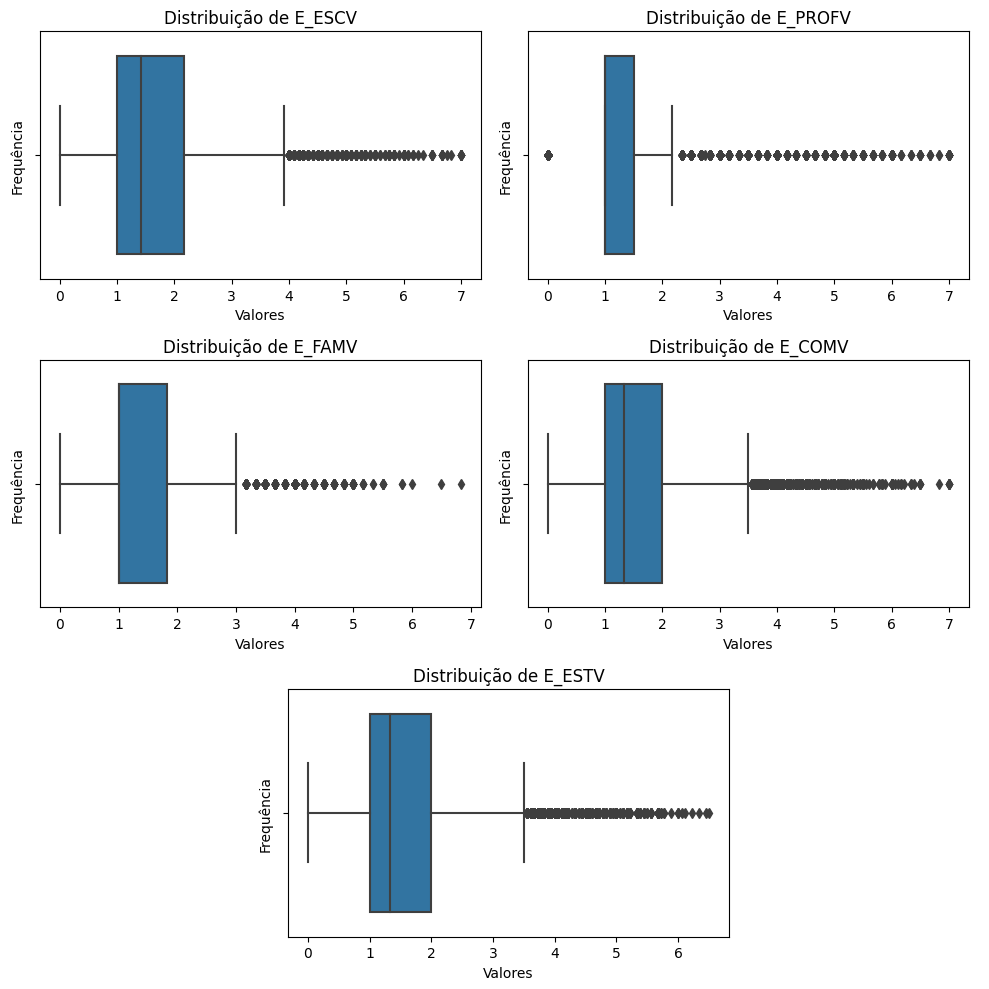
\includegraphics[width=0.8\textwidth]{Textuais/Imagens/Gráficos/boxplot_dim.png}
    \label{fig:box_plot_dimensoes}
    \fonte{\me{2023}}
\end{figure}



\begin{figure}[ht!]
    \centering
    \caption{Box Plot de distribuição de Fatores}
    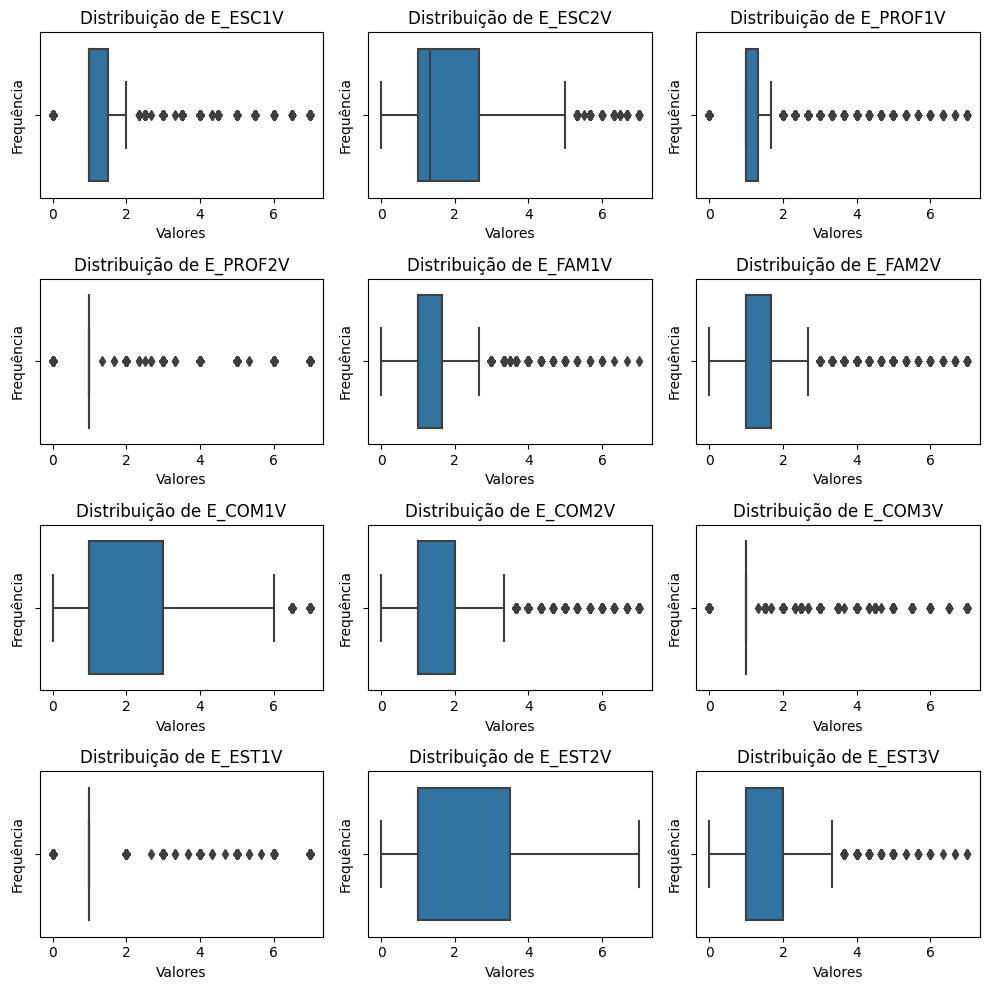
\includegraphics[width=0.8\textwidth]{Textuais/Imagens/Gráficos/boxplot_fat.png}
    \label{fig:box_plot_fatores}
    \fonte{\me{2023}}
\end{figure}




% As tabelas apresentam estatísticas descritivas relacionadas a fatores e dimensões de um questionário. Vamos analisar as conclusões possíveis com base nos números fornecidos:

% \textbf{Tabela de Estatísticas de Fatores:}

% \begin{enumerate}
%     \item E\_ESC1V tem uma média de aproximadamente 1.57, um desvio padrão de cerca de 1.19 e uma mediana de 1. Isso indica que a maioria das respostas está próxima da mediana, com uma dispersão moderada. Parece haver uma variedade razoável de respostas.
%     \item E\_ESC2V tem uma média de cerca de 1.93, um desvio padrão de aproximadamente 1.19 e uma mediana de 1.33. Isso sugere que as respostas estão distribuídas de forma um pouco mais ampla em comparação com E\_ESC1V, com uma mediana ligeiramente maior.
%     \item E\_PROF1V tem uma média de cerca de 1.39, um desvio padrão de aproximadamente 0.93 e uma mediana de 1. Parece haver menos dispersão nas respostas, com a maioria dos dados próximos à mediana.
%     \item E\_PROF2V tem uma média de aproximadamente 1.62, um desvio padrão de cerca de 1.60 e uma mediana de 1. A dispersão é alta, com uma mediana baixa, sugerindo uma variedade significativa de respostas.
%     \item E\_FAM1V tem uma média de cerca de 1.43, um desvio padrão de aproximadamente 0.79 e uma mediana de 1. As respostas parecem estar concentradas perto da mediana, com uma dispersão moderada.
%     \item E\_FAM2V tem uma média de aproximadamente 1.52, um desvio padrão de cerca de 1.06 e uma mediana de 1. A dispersão é moderada, e a mediana é próxima de 1, indicando que a maioria das respostas está nessa faixa.
%     \item E\_COM1V tem uma média de cerca de 2.01, um desvio padrão de aproximadamente 1.59 e uma mediana de 1. Isso indica uma dispersão considerável nas respostas, com uma mediana relativamente baixa.
%     \item E\_COM2V tem uma média de cerca de 1.60, um desvio padrão de aproximadamente 1.12 e uma mediana de 1. Parece haver uma variedade razoável nas respostas, com a maioria próxima à mediana.
%     \item E\_COM3V tem uma média de cerca de 1.35, um desvio padrão de aproximadamente 0.96 e uma mediana de 1. A dispersão é moderada, e a mediana está próxima de 1.
%     \item E\_EST1V tem uma média de cerca de 1.39, um desvio padrão de aproximadamente 1.22 e uma mediana de 1. A dispersão é moderada, com a maioria das respostas próximas à mediana.
%     \item E\_EST2V tem uma média de aproximadamente 2.03, um desvio padrão de cerca de 1.57 e uma mediana de 1. A dispersão é alta, e a mediana está próxima de 1.
%     \item E\_EST3V tem uma média de cerca de 1.53, um desvio padrão de aproximadamente 0.84 e uma mediana de 1. A dispersão é moderada, e a mediana está próxima de 1.
%     \end{enumerate}

    
% \textbf{Tabela de Estatísticas de Dimensões:}

% \begin{enumerate}
%     \item E\_ESCV tem uma média de aproximadamente 1.76, um desvio padrão de cerca de 0.96 e uma mediana de 1.42. Isso indica que a dimensão ``Estudante – Escola'' (E-ESC) tem uma dispersão moderada, com a maioria das respostas próxima à mediana.
    
%     \item E\_PROFV tem uma média de cerca de 1.50, um desvio padrão de aproximadamente 1.07 e uma mediana de 1. A dispersão é moderada, e a mediana está próxima de 1, sugerindo uma consistência nas respostas.
    
%     \item E\_FAMV tem uma média de aproximadamente 1.49, um desvio padrão de cerca de 0.78 e uma mediana de 1. A dimensão ``Estudante – Família'' (E-FAM) apresenta uma dispersão moderada, com a maioria das respostas próxima à mediana.
    
%     \item E\_COMV tem uma média de cerca de 1.68, um desvio padrão de aproximadamente 0.87 e uma mediana de 1.33. A dimensão ``Estudante – Comunidade'' (E-COM) tem uma dispersão moderada, com uma mediana acima de 1.
    
%     \item E\_ESTV tem uma média de aproximadamente 1.67, um desvio padrão de cerca de 0.86 e uma mediana de 1.33. A dimensão ``Estudante – Estudante'' (E-EST) apresenta uma dispersão moderada, com a maioria das respostas próxima à mediana. 
% \end{enumerate}
% Em resumo, as estatísticas fornecidas indicam a variabilidade nas respostas dos participantes do questionário, com algumas dimensões e fatores apresentando maior dispersão do que outras. É importante considerar esses resultados ao analisar os dados e as respostas do questionário em um contexto mais amplo.


%%%%%%%%%%%%%%%%%%%%%%%%%%%%%%%%%%%%%%%%%
%%%%%%%%%%%%%%%%%%%%%%%%%%%%%%%%%%%%%%%%%


A Figura \ref{fig:uf} apresenta o mapa temático do Brasil, colorido em diferentes tons que representam a quantidade de estudantes por estado que responderam ao questionário. A barra de cores à direita do mapa serve como uma legenda, indicando a relação entre as cores e o número de estudantes, com a escala variando do amarelo claro para números baixos até o vermelho escuro para números altos.

Há uma grande variação na quantidade de respostas por estado. Alguns estados, como o destacado em vermelho escuro no centro-norte do mapa, têm um número significativamente alto de estudantes respondentes, ultrapassando 5000. Isso sugere uma alta participação ou um foco particular na coleta de dados nesse estado. Por outro lado, há estados, especialmente no sul do país, que apresentam números baixos ou nulos, indicando uma possível falta de representatividade ou dificuldades na coleta de dados nessas áreas.

Além disso, o mapa fornece informações sobre onde podem estar concentradas as preocupações com a evasão, ou pelo menos onde mais estudantes foram alcançados para responder ao questionário. A heterogeneidade na distribuição dos números pode refletir diferenças no engajamento das secretarias de educação estaduais, na estrutura da pesquisa, ou até mesmo na própria incidência de evasão escolar.

\begin{figure}[ht!]
    \centering
    \caption{Distribuição das matrículas por estados}
    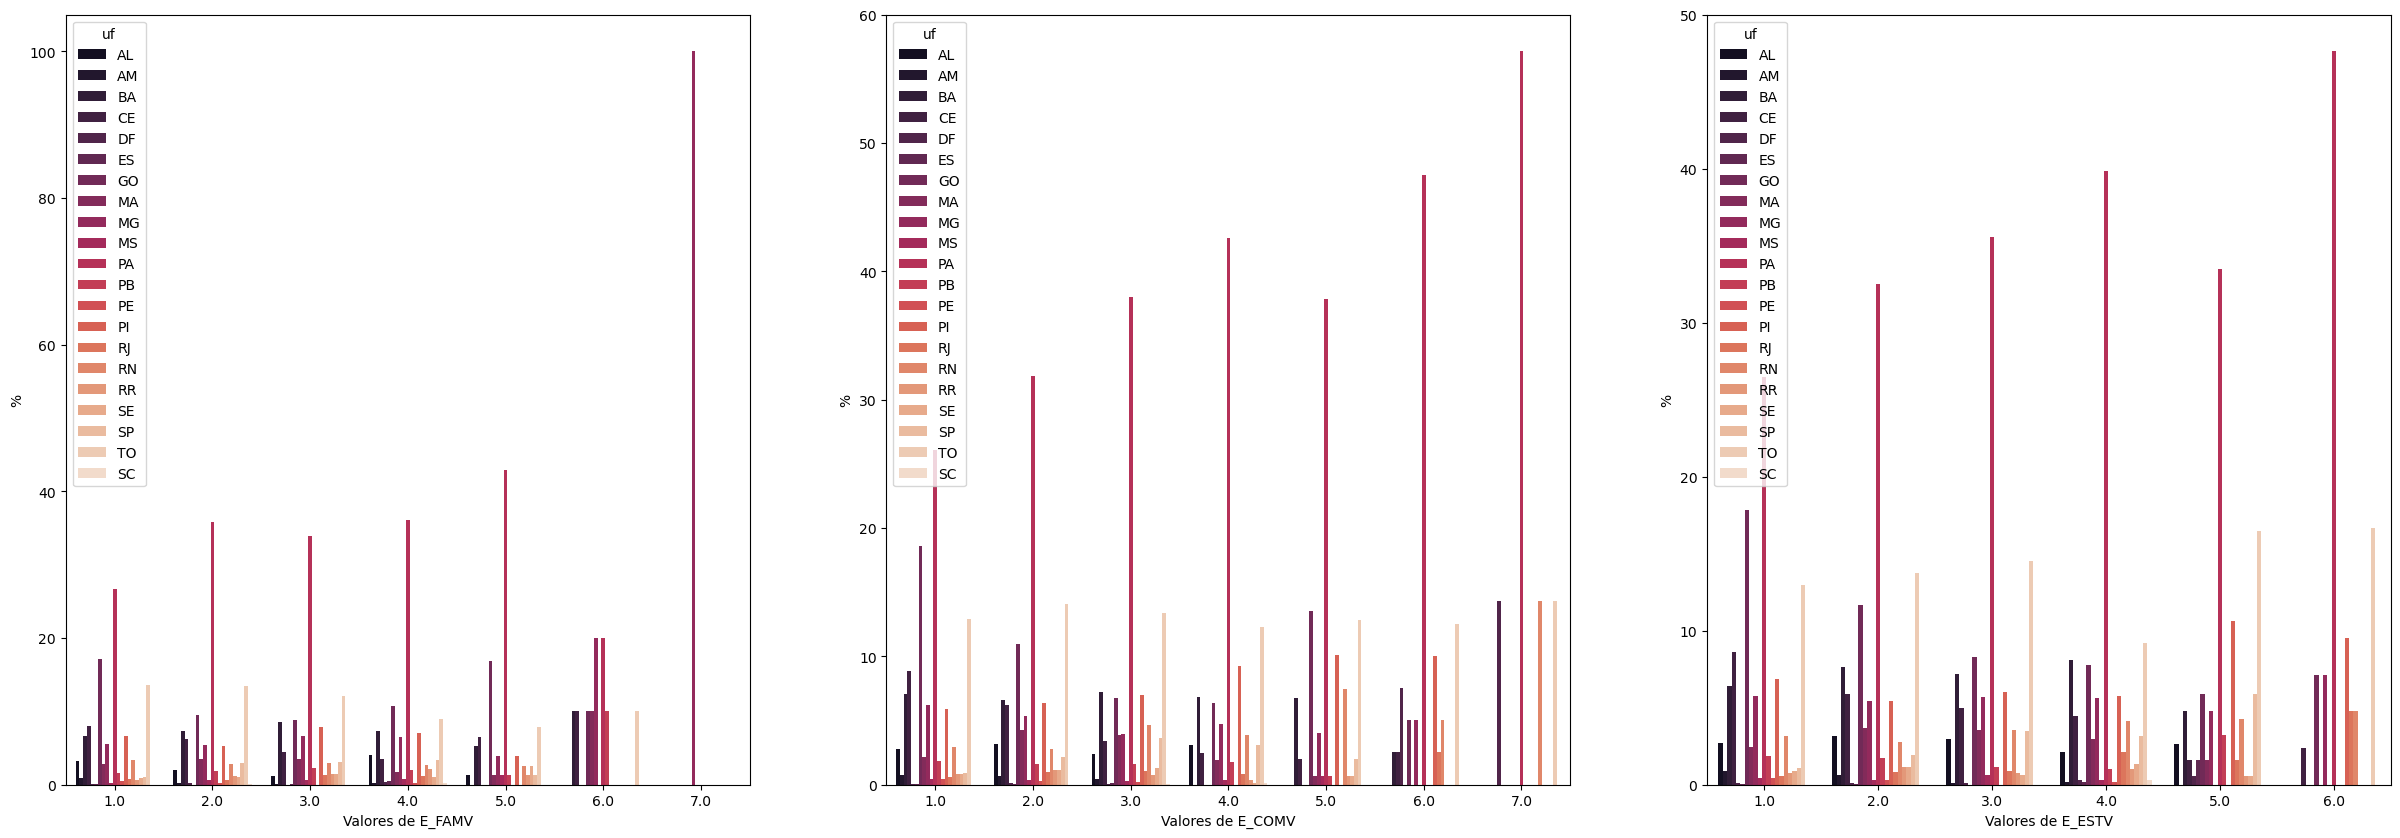
\includegraphics[width=\textwidth]{Textuais/Imagens/Gráficos/uf.png}
    \label{fig:uf}
\end{figure}

O gráfico da Figura \ref{fig:turmas} exibe a distribuição do número de estudantes que responderam ao questionário categorizados por ano escolar. Observa-se que a maior participação foi dos alunos do 6º ano, com 4912 respostas, seguida por uma ligeira diminuição para 4418 no 7º ano e uma redução mais acentuada para 4103 no 8º ano. O 9º ano apresenta um número ainda menor de respondentes, com 3506 alunos. Uma queda drástica é notada nos anos iniciais do ensino fundamental: apenas 61 estudantes do 5º ano, 59 do 1º ano, 23 do 3º ano, 18 do 2º ano e 9 do 4º ano participaram do questionário.

\begin{figure}[ht!]
    \centering
    \caption{Distribuição das matrículas por ano de turma do ensino fundamental}
    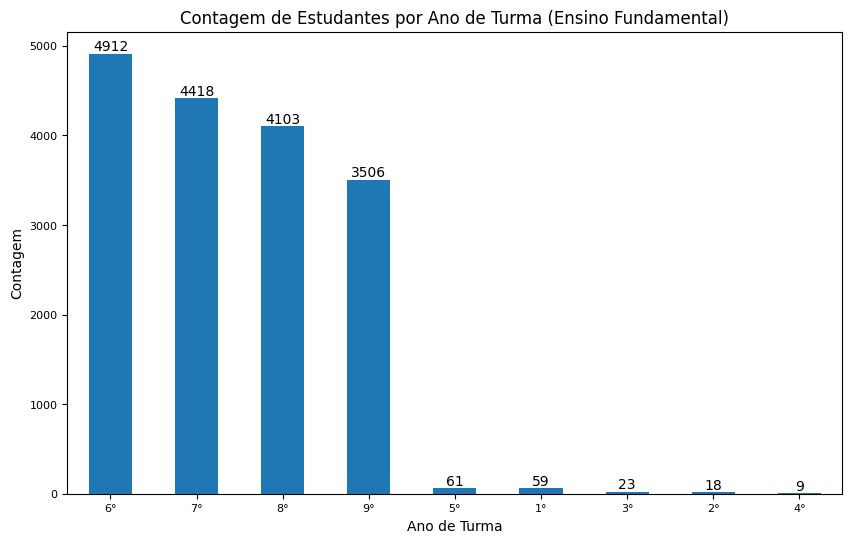
\includegraphics[width=0.8\textwidth]{Textuais/Imagens/Gráficos/turmas.png}
    \label{fig:turmas}
    \fonte{\me{2023}}
\end{figure}

O gráfico da Figura \ref{fig:sexo-porcent} é um gráfico de pizza que apresenta a distribuição por sexo dos estudantes que responderam o questionário. Do total de respondentes, 51,7\% são do sexo masculino e 48,3\% do sexo feminino. Isso indica uma distribuição quase equilibrada entre os gêneros, com uma ligeira predominância de respondentes masculinos. 

\begin{figure}[ht!]
    \centering
    \caption{Porcentagem do sexo dos estudantes}
    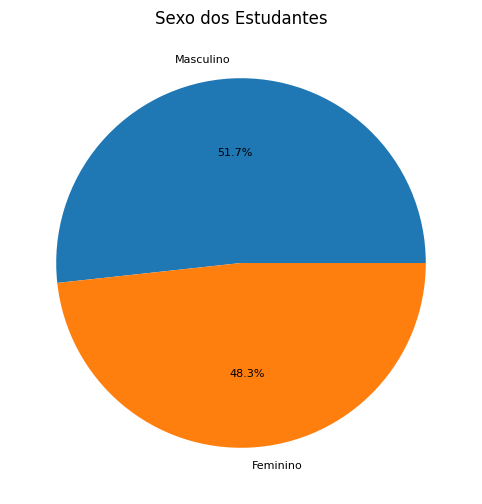
\includegraphics[width=0.6\textwidth]{Textuais/Imagens/Gráficos/sexo.png}
    \label{fig:sexo-porcent}
    \fonte{\me{2023}}
\end{figure}

% A renda familiar pode exercer uma influência significativa na permanência do estudante na escola devido a vários fatores. Estudantes de famílias com rendas mais baixas podem enfrentar dificuldades econômicas que os obrigam a priorizar o trabalho imediato em detrimento da educação continuada. Essa necessidade de contribuir para a renda da família pode levar à evasão escolar, já que o estudante pode ter que dedicar seu tempo a atividades remuneradas.

% Além disso, a limitação de recursos financeiros pode afetar a capacidade de uma família de pagar por materiais didáticos, uniformes, transporte e outras despesas educacionais. Isso pode resultar em uma experiência educacional de qualidade inferior, com menos apoio e recursos, o que, por sua vez, pode desmotivar o estudante e aumentar as chances de evasão escolar.

% Outro aspecto é o acesso a uma educação de qualidade. Em muitos casos, escolas localizadas em regiões de baixa renda podem estar superlotadas, mal equipadas e com menos oportunidades extracurriculares, o que pode afetar negativamente o engajamento e o desempenho do estudante. Estudantes de famílias com maior renda, em contraste, muitas vezes têm acesso a escolas privadas ou públicas bem financiadas, com uma ampla gama de programas de apoio, como tutoria e aconselhamento, que podem ajudar a mantê-los na escola.

% De acordo com um estudo realizado por Reardon et. al (2016)\nocite{reardon2019geography}, a renda familiar está fortemente associada às oportunidades educacionais e ao desempenho acadêmico. O estudo descobriu que, nos Estados Unidos, a lacuna de desempenho entre crianças de famílias de baixa renda e crianças de famílias de alta renda é significativa e tem aumentado ao longo do tempo. As crianças de famílias de baixa renda têm menos acesso a recursos educacionais, como escolas de alta qualidade, professores experientes e programas extracurriculares, o que pode afetar negativamente suas expectativas e aspirações educacionais. Além disso, as famílias de baixa renda podem ter menos recursos financeiros para investir na educação de seus filhos, o que pode limitar suas oportunidades educacionais a longo prazo.


% Portanto, é possível afirmar que a renda familiar influencia diretamente as expectativas educacionais e os resultados a longo prazo, uma vez que as famílias com maior renda geralmente têm mais recursos para apoiar a educação de seus filhos, enquanto as famílias de baixa renda podem enfrentar desafios financeiros e ter menos acesso a recursos educacionais.

% Políticas e programas focados em aumentar o apoio financeiro para famílias de baixa renda, fornecer recursos educacionais adicionais, e criar oportunidades de ensino pós-escolar podem ser cruciais para reduzir as taxas de evasão escolar e promover a igualdade educacional.

Desta forma, o gráfico da Figura \ref{fig:renda_fam} apresenta a distribuição de renda das famílias dos estudantes respondentes. A maior concentração de estudantes, 8.735, tem uma renda familiar de até 1 salário mínimo (até R\$ 1.320). A segunda maior faixa, com 5.222 estudantes, situa-se entre 1 a 3 salários mínimos (de R\$ 1.320 até R\$ 3.960). Uma parcela considerável, 2.130 estudantes, indicou não possuir nenhuma renda. A faixa de 4 a 6 salários mínimos (de R\$ 5.280 até R\$ 7.920) é composta por 816 estudantes. Observa-se uma diminuição progressiva na quantidade de estudantes à medida que a renda familiar aumenta: 139 estudantes pertencem à faixa de 7 a 9 salários mínimos (de R\$ 9.240 até R\$ 11.880), e apenas 67 estudantes têm uma renda familiar acima de 9 salários mínimos (mais de R\$ 11.880). Esse perfil sugere que a maioria dos estudantes que participaram do questionário provém de famílias com menor renda.


\begin{figure}[ht!]
    \centering
    \caption{Distribuição de renda da família dos estudantes}
    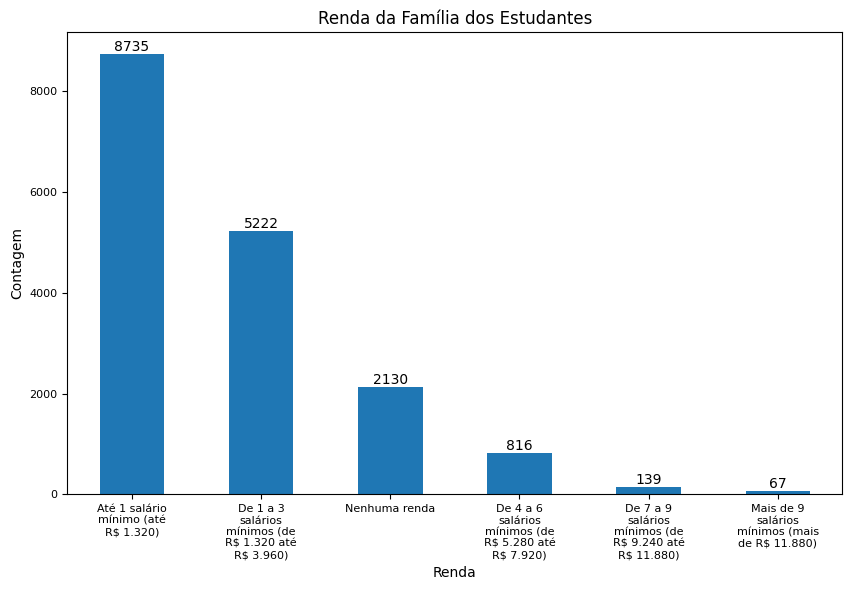
\includegraphics[width=0.8\textwidth]{Textuais/Imagens/Gráficos/renda_fam.png}
    \label{fig:renda_fam}
    \fonte{\me{2023}}
\end{figure}


% A oferta de Atendimento Educacional Especializado (AEE) é uma prática inclusiva essencial que visa atender às necessidades específicas de estudantes com deficiência, transtornos globais do desenvolvimento ou altas habilidades/superdotação. Quando as escolas fornecem esse tipo de suporte especializado, elas não apenas ajudam a nivelar o campo de jogo educacional para esses alunos, mas também promovem uma cultura de inclusão e igualdade. A presença de serviços de AEE pode aumentar significativamente as chances de retenção dos estudantes na escola, uma vez que se sentem apoiados em suas necessidades educacionais particulares e, consequentemente, mais engajados e motivados para continuar seus estudos.

% Por outro lado, as atividades complementares, que podem incluir clubes, esportes, música, arte, e outras experiências enriquecedoras, desempenham um papel vital na educação holística dos alunos. Essas atividades são fundamentais para o desenvolvimento de habilidades sociais, emocionais e cognitivas. Alunos que participam dessas atividades tendem a desenvolver um senso de pertencimento e compromisso com sua comunidade escolar. A disponibilidade de tais programas pode influenciar positivamente a decisão de um aluno de permanecer na escola, pois eles proporcionam uma saída para a expressão criativa, alívio do estresse e oportunidades para amizades e mentorias. Além disso, as atividades complementares aumentam frequentemente o engajamento dos alunos com o ambiente escolar e podem melhorar o desempenho acadêmico, tornando a experiência educacional mais atraente e valiosa.

% A combinação dessas ofertas indica que a escola está buscando atender a uma gama diversificada de necessidades dos alunos, tanto educacionais quanto de desenvolvimento pessoal. Tais esforços multidimensionais são fundamentais para a retenção de estudantes, pois eles se sentem compreendidos e atendidos em suas demandas individuais. Ao considerar o aspecto multidisciplinar do desenvolvimento do estudante e suas variadas necessidades, a escola pode reduzir os índices de evasão e fomentar uma comunidade escolar mais integrada e resiliente.

O gráfico da Figura \ref{fig:outras_ofertas} apresenta a distribuição de frequência de estudantes em relação a três categorias distintas de Outras Ofertas Educacionais. Observa-se que a maior frequência está na categoria ``Atendimento Educacional Especializado'', com 5646 estudantes. Isso indica que esta é a oferta educacional mais acessada ou necessitada pelo grupo de estudantes que respondeu ao questionário. Em seguida, temos a ``Atividade Complementar'', com 1615 estudantes, demonstrando uma procura ou necessidade significativamente menor em comparação à primeira. Por fim, a categoria ``Atendimento Educacional Especializado, Atividade Complementar'' registra 1212 estudantes, sugerindo que há um número considerável de estudantes que necessitam ou acessam uma combinação das ofertas. 

\begin{figure}[ht!]
    \centering
    \caption{Número de estudantes que estão matriculados em instituições que possuem ofertas educacionais diferenciadas}
    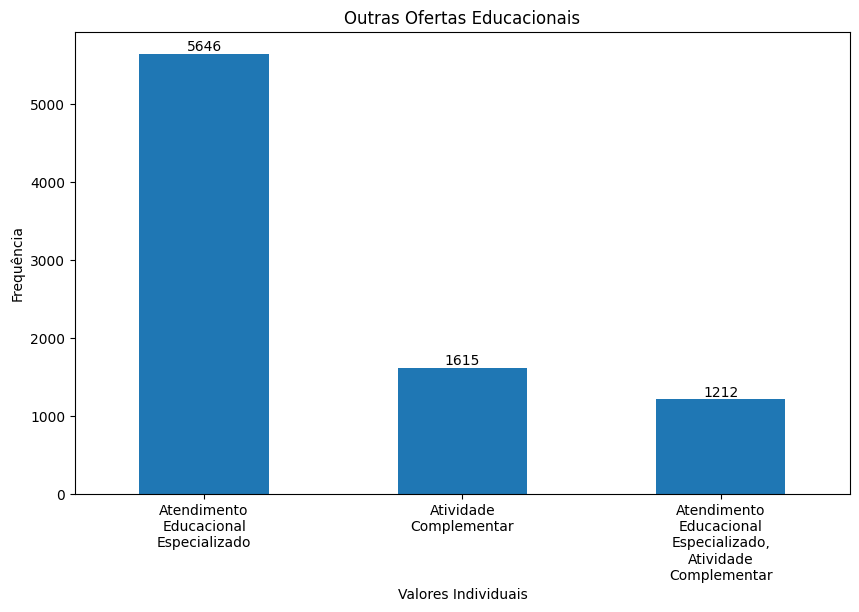
\includegraphics[width=0.8\textwidth]{Textuais/Imagens/Gráficos/outras_ofertas_educacionais.png}
    \label{fig:outras_ofertas}
    \fonte{\me{2023}}
\end{figure}



% A localização das escolas, seja em áreas rurais ou urbanas, pode influenciar significativa na permanência dos estudantes na escola. Em áreas urbanas, os estudantes costumam ter acesso a uma gama mais ampla de recursos educacionais, como tecnologia mais avançada, maior número de professores qualificados, e uma variedade maior de programas extracurriculares e de apoio ao aluno. Esses fatores podem contribuir para uma maior taxa de retenção de alunos, já que eles têm mais oportunidades de engajamento e aprendizado. Além disso, escolas urbanas muitas vezes estão mais próximas dos serviços de apoio ao estudante, como bibliotecas públicas e centros de tutoria \cite{santos2012estudo}. 


% Por outro lado, escolas localizadas em áreas rurais podem enfrentar desafios distintos que impactam a permanência do estudante. O acesso limitado a recursos, como Internet de alta velocidade e materiais didáticos atualizados, pode afetar a qualidade da educação. Distâncias maiores para se percorrer até a escola e a falta de transporte público adequado são problemas comuns que podem levar a altas taxas de evasão, pois tornam o simples ato de chegar à escola um desafio. Além disso, em muitas comunidades rurais, pode haver uma expectativa maior de que os jovens contribuam para o trabalho familiar, o que pode priorizar as necessidades de trabalho em detrimento da educação formal.

% Outra consideração é o impacto econômico e cultural das áreas rurais e urbanas. Em regiões rurais, pode haver menos incentivo para a educação de longo prazo se as oportunidades de emprego local forem limitadas ou se valorizarem mais as habilidades práticas adquiridas fora do ambiente escolar. Em contrapartida, áreas urbanas tendem a oferecer uma maior variedade de oportunidades profissionais que requerem educação formal, incentivando os estudantes a concluírem seus estudos.

% De acordo com o Observatório da Criança e do Adolescente, a média de horas-aula no Ensino Fundamental varia de acordo com a localização da escola, sendo que a média de horas-aula expressa o tempo médio de permanência dos alunos na escola segundo a localização (urbana ou rural) do estabelecimento de ensino. A média apresentada é ponderada por fator que deriva das relações entre: a matrícula na data de referência do Censo Escolar, a série, os grupos de séries e níveis de ensino. Para este indicador são consideradas apenas as turmas de escolarização na modalidade Regular \footnote{https://observatoriocrianca.org.br/cenario-infancia/temas/ensino-fundamental/883-media-de-horas-aula-no-ensino-fundamental-segundo-localizacao-urbana-e-rural?filters=1,1385}.
% Além disso, a quantidade de horas-aula modifica conforme a localidade da escola, apresentando um número menor em escolas de área rural.

% Por fim, políticas públicas e investimentos em educação podem variar consideravelmente entre áreas rurais e urbanas, afetando diretamente a permanência dos estudantes na escola. Iniciativas para melhorar a infraestrutura escolar, oferecer transporte aos estudantes e programas de incentivo à permanência na escola são essenciais para garantir que a localização geográfica não seja uma barreira à educação. Reconhecer e abordar essas diferenças é fundamental para qualquer estratégia que vise diminuir a evasão escolar e promover a igualdade de acesso à educação de qualidade para todos os estudantes.


Já o gráfico da Figura \ref{fig:localizacao} mostra a localização das escolas de acordo com as respostas dos estudantes. De acordo com as informações fornecidas, 59,2\% dos estudantes estão em escolas localizadas em áreas urbanas, enquanto os restantes 40,8\% estão em escolas situadas em áreas rurais. Isso indica uma distribuição relativamente equilibrada entre as localizações das escolas dos respondentes, com uma ligeira predominância de estudantes em zonas urbanas. Na Tabela \ref{tab:localizacao_escolas_estado}, foi realizada a separação do número de escolas e sua localização por cada estado, querendo analisar melhor da distribuição de escolas rurais e urbanas no âmbito nacional. É possível observar que a maioria dos estados possui maior concentração urbana, exceto pelos estados de Alagoas, Bahia, Maranhão, Pará e Rio Grande do Norte.

\begin{figure}[ht!]
    \centering
    
    \caption{Porcentagem da localização das escolas}
    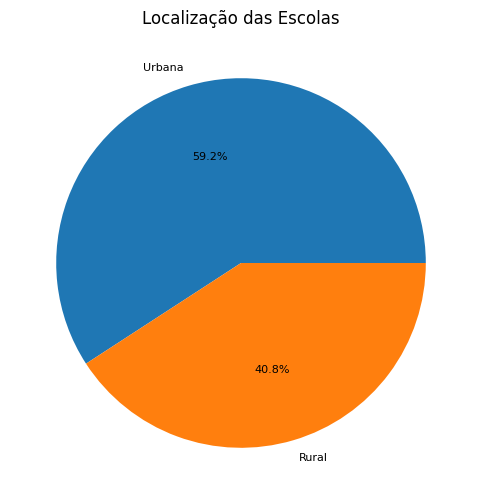
\includegraphics[width=0.6\textwidth]{Textuais/Imagens/Gráficos/localizacao.png}
    \label{fig:localizacao}
    \fonte{\me{2023}}
\end{figure}

\begin{table}[ht!]
\centering
\caption{Localização das escolas dividida por estado}
\label{tab:localizacao_escolas_estado}
\resizebox{\textwidth}{!}{%
\begin{tabular}{|c|c|c|c|c|c|c|c|c|c|c|c|c|c|c|c|c|c|c|c|c|c|}
\hline
\textbf{UF}                               & AL & AM & BA & CE & DF & ES & GO & MA & MG & MS & PA & PB & PE & PI & RJ & RN & RR & SC & SE & SP & TO \\ \hline
\textbf{Rural}                            & 4  & 1  & 17 & 7  & 0  & 0  & 1  & 14 & 5  & 0  & 68 & 1  & 1  & 5  & 0  & 6  & 0  & 0  & 1  & 1  & 15 \\ \hline
\textbf{Urbana} & 3  & 1  & 9  & 12 & 1  & 1  & 28 & 7  & 9  & 2  & 33 & 3  & 1  & 11 & 2  & 2  & 4  & 1  & 4  & 4  & 23 \\ \hline
\end{tabular}%
}
\fonte{\me{2023}}
\end{table}

% A localidade de uma escola pode exercer um papel crucial na permanência do estudante na instituição. Em áreas de assentamento, por exemplo, os estudantes podem enfrentar desafios como acesso limitado ao transporte, recursos educacionais escassos ou infraestrutura inadequada, o que pode contribuir para altas taxas de evasão escolar. Estes assentamentos estão frequentemente situados em locais remotos, onde as escolas podem lutar para atrair e reter professores qualificados, e os alunos podem ter que viajar longas distâncias para frequentar as aulas, o que pode ser um impedimento significativo à regularidade da frequência escolar.

% Em áreas remanescentes de quilombos, as escolas estão muitas vezes inseridas em comunidades com raízes históricas e culturais. Embora isso possa fornecer um ambiente de aprendizado rico culturalmente, também pode haver desafios devido ao isolamento geográfico e à falta de recursos. Questões como a relevância cultural do currículo e a sensibilidade dos professores às tradições locais podem influenciar a decisão do estudante de continuar na escola. Nas terras indígenas, a situação é muitas vezes mais complexa, pois envolve a preservação da língua e da cultura indígenas, além dos desafios de infraestrutura e acessibilidade. A educação nessas áreas pode ser dificultada por políticas governamentais inadequadas ou pela falta de material didático que incorpore a língua e a cultura indígenas. A relevância cultural do ensino é um fator determinante para a permanência do estudante, e a falta dela pode levar à desmotivação e ao abandono escolar.

O gráfico apresentado na Figura \ref{fig:localidades} é um diagrama de barras que exibe a distribuição de escolas por tipos de localidades diferenciadas. Três categorias são exibidas: ``Área de assentamento'', ``Área remanescente de quilombos'' e ``Terra indígena''. A maior contagem de escolas, com um total de 25, encontra-se em ``Área de assentamento''. Em segundo lugar, com 8 escolas, estão as ``Áreas remanescentes de quilombos''. Por fim, ``Terra indígena'' apresenta 4 escolas. Considerando o gráfico da Figura \ref{fig:localidades_brasil}, feito com os dados do Novo Censo Educacional exclusivos do ano de 2022\footnote{https://www.gov.br/inep/pt-br/acesso-a-informacao/dados-abertos/microdados/censo-escolar}, nota-se que a proporcionalidade das escolas pesquisadas que estão em localizações diferenciadas não foi igual na pesquisa do SAP. Sabendo que foram pesquisadas 224.649 escolas no Censo, os resultados mostram que a porcentagem de escolas com localizações em área de assentamento, terras indígenas e áreas remanescentes de quilombos era 2.03\%, 1.5\% e 1.14\%, respectivamente. Já no SAP, essas mesmas categorias possuem porcentagens de 8.11\%, 1.29\% e 2.59\%; ou seja, o dobro para remanescentes.

\begin{figure}[ht!]
    \centering
    \caption{Localização diferenciada das escolas}
    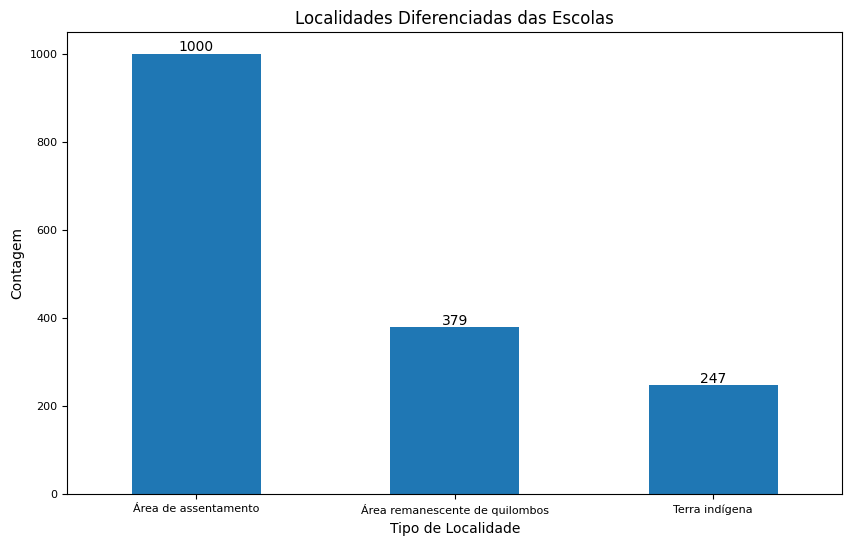
\includegraphics[width=0.8\textwidth]{Textuais/Imagens/Gráficos/localidadesdifer.png}
    \label{fig:localidades}
    \fonte{\me{2023}}
\end{figure}

\begin{figure}[ht!]
    \centering
    \caption{Localização diferenciada das escolas brasileiras no ano de 2022}
    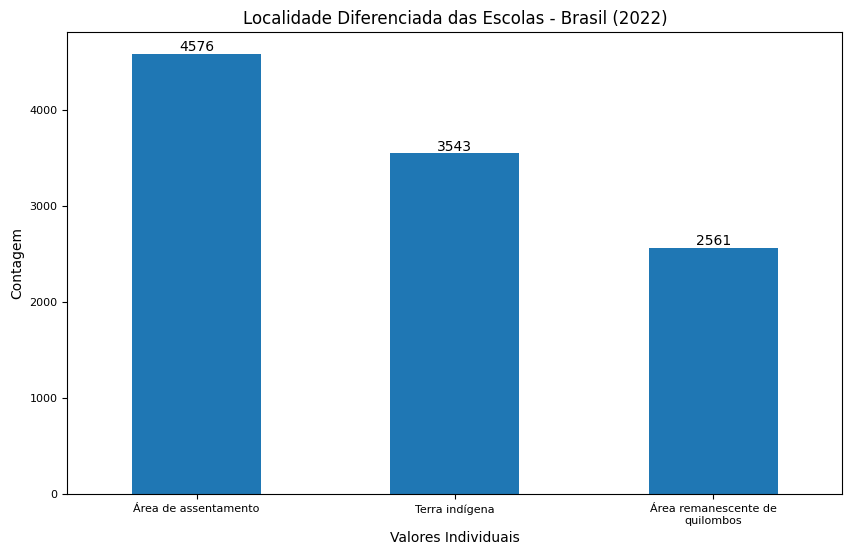
\includegraphics[width=0.8\textwidth]{Textuais/Imagens/Gráficos/localidadesdifer_brasil.png}
    \label{fig:localidades_brasil}
    \fonte{\me{2023}}
\end{figure}

% A faixa do número de matrículas em uma escola pode ter diversas implicações na permanência dos estudantes, influenciando diretamente a qualidade da educação e o ambiente escolar. Em escolas com um número elevado de matrículas, que muitas vezes correspondem a escolas de maior porte, pode haver acesso a mais recursos, como bibliotecas mais amplas, maior variedade de atividades extracurriculares e infraestrutura esportiva. Isso pode aumentar o engajamento dos alunos e diminuir as chances de evasão. No entanto, o grande número de estudantes pode também levar a uma menor atenção individual por parte dos professores e funcionários, o que pode afetar negativamente os alunos que necessitam de maior suporte pedagógico. Por outro lado, escolas com poucas matrículas podem proporcionar um ambiente mais acolhedor e personalizado, com maior proximidade entre alunos e professores. Nesses ambientes, os educadores podem acompanhar mais de perto o progresso e as dificuldades de cada aluno, o que pode ser decisivo na prevenção da evasão escolar. No entanto, essas escolas podem enfrentar limitações de recursos, o que poderia afetar a oferta de cursos e atividades e, por conseguinte, o interesse dos alunos em permanecer na escola.

O gráfico da Figura \ref{fig:faixa_num} ilustra a distribuição do número de matrículas das escolas. O eixo horizontal representa diferentes faixas de número de matrículas, enquanto o eixo vertical indica a contagem de escolas em cada faixa. A maior concentração de escolas se encontra na faixa de ``Entre 51 e 200'' matrículas, com um total de 92 escolas. Segue-se a faixa de ``Entre 501 e 1000'' matrículas com 67 escolas, e ``Mais de 1000'' com 21 escolas. Por fim, o número de escolas com ``Até 50'' matrículas é o mais baixo, com apenas 5 instituições. Este gráfico traz o entendimento da distribuição do tamanho das escolas entre os estudantes que participaram do questionário, o que pode fornecer uma visão mais completa para a análise da evasão escolar.

\begin{figure}[ht!]
    \centering
    \caption{Faixa do número de matrículas das escolas}
    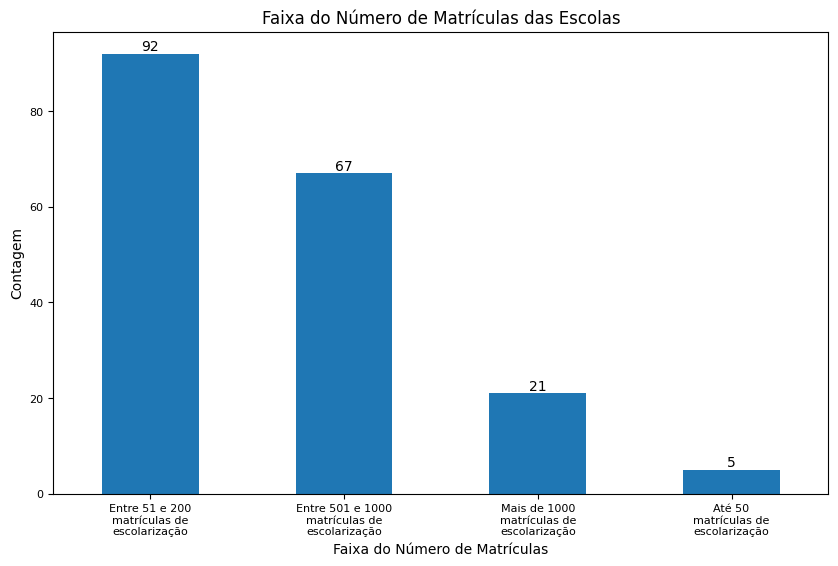
\includegraphics[width=0.8\textwidth]{Textuais/Imagens/Gráficos/faixanumamatr.png}
    \label{fig:faixa_num}
    \fonte{\me{2023}}
\end{figure}

A etnia dos estudantes está relacionada a uma complexa teia de fatores sociais, econômicos e culturais. Estudantes identificados como pardos, pretos, indígenas e amarelos podem enfrentar desafios adicionais que afetam sua jornada educacional. Questões como disparidades socioeconômicas, preconceito e racismo estrutural podem influenciar negativamente a experiência desses estudantes nas instituições de ensino \cite{heringer2018democratizaccao}. O gráfico apresentado na Figura \ref{fig:etnia} mostra a distribuição étnica dos estudantes que responderam o questionário. A categoria com maior número de estudantes é a ``Pardo/a'', com 12.450 respostas, seguida consideravelmente pela categoria ``Branco/a'' com 2.443 estudantes. A terceira categoria mais numerosa é a ``Preto/a'', representando 1.758 estudantes. Em menor quantidade, aparecem os estudantes que se identificam como ``Indígena'', somando 290, e a categoria ``Amarelo/a (Origem Asiática)'' com 168 estudantes. A representação visual destes dados permite uma compreensão imediata das proporções relativas de cada grupo étnico dentro do conjunto dos respondentes, destacando a predominância do grupo ``Pardo/a'' neste contexto específico.

Observando os microdados das etnias do Censo da Educação Básica do ano de 2022, apresentados na Figura \ref{fig:etnia-brasil}, nota-se que proporcionalmente, os números de representatividade das etnias são muito semelhantes, com a exceção dos declarados brancos e dos estudantes não declarados, que no Censo são o terceiro maior grupo, mas que no SAP não é bem uma categoria existente, indicando que todos os 17110 respondentes declararam suas etnias.

% Para estudantes pardos e pretos, por exemplo, a marginalização histórica e contínua pode levar a menores investimentos em suas comunidades e escolas, resultando em acesso desigual a recursos educacionais de qualidade. Além disso, o racismo e a discriminação podem criar ambientes escolares hostis, reduzindo o senso de pertencimento e segurança desses alunos, o que pode aumentar as taxas de evasão.

% De acordo com a pesquisa realizada pelo Observatório de Educação do Instituto Unibanco\footnote{https://observatoriodeeducacao.institutounibanco.org.br/em-debate/desigualdade-racial-na-educacao}, a marginalização histórica e contínua pode levar a menores investimentos em comunidades e escolas, resultando em acesso desigual a recursos educacionais de qualidade para estudantes pardos e pretos. Além disso, o racismo e a discriminação podem criar ambientes escolares hostis, reduzindo o senso de pertencimento e segurança desses alunos, o que pode aumentar as taxas de evasão

% Estudantes indígenas muitas vezes enfrentam barreiras ainda maiores, como a distância física de suas comunidades para as escolas, a falta de materiais didáticos que respeitem e reflitam suas culturas e línguas, e um modelo educacional que frequentemente não leva em conta suas tradições e saberes.

% Conforme o ensaio ``O passado e o futuro da educação indígena: barreiras e soluções'' do \textit{Indigenous Brazil}\footnote{https://commons.princeton.edu/indigenous-brazil/outros-textos/o-passado-e-o-futuro-da-educacao-indigena-barreiras-e-solucoes/}, estudantes indígenas enfrentam barreiras ainda maiores, como a distância física de suas comunidades para as escolas, a falta de materiais didáticos que respeitem e reflitam suas culturas e línguas, e um modelo educacional que frequentemente não leva em conta suas tradições e saberes

% Por outro lado, estudantes amarelos, que podem incluir descendentes de imigrantes asiáticos, podem experimentar estereótipos tanto positivos quanto negativos que afetam suas experiências educacionais. Embora muitas vezes sejam vistos sob a ``lente do modelo minoritário'', que pressupõe um alto desempenho acadêmico, eles também podem enfrentar isolamento cultural e racismo.

% Estudantes brancos, em muitos contextos, podem ter vantagens devido a privilégios estruturais que lhes concedem melhor acesso a escolas de alta qualidade, materiais didáticos e oportunidades extracurriculares. Contudo, isso não significa que estudantes brancos não enfrentem desafios que possam influenciar sua permanência na escola; fatores como condição socioeconômica e outras questões individuais ou familiares também são relevantes.



\begin{figure}[ht!]
    \centering
    \caption{Etnias dos estudantes que responderam o IAFREE}
    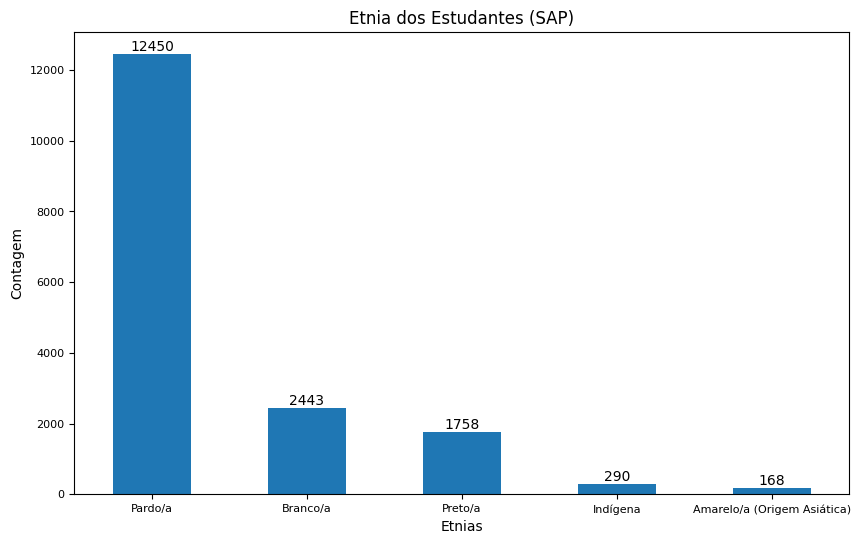
\includegraphics[width=0.8\textwidth]{Textuais/Imagens/Gráficos/etnia.png}
    \label{fig:etnia}
    \fonte{\me{2023}}
\end{figure}

\begin{figure}[ht!]
    \centering
    \caption{Etnias dos estudantes - Censo 2022}
    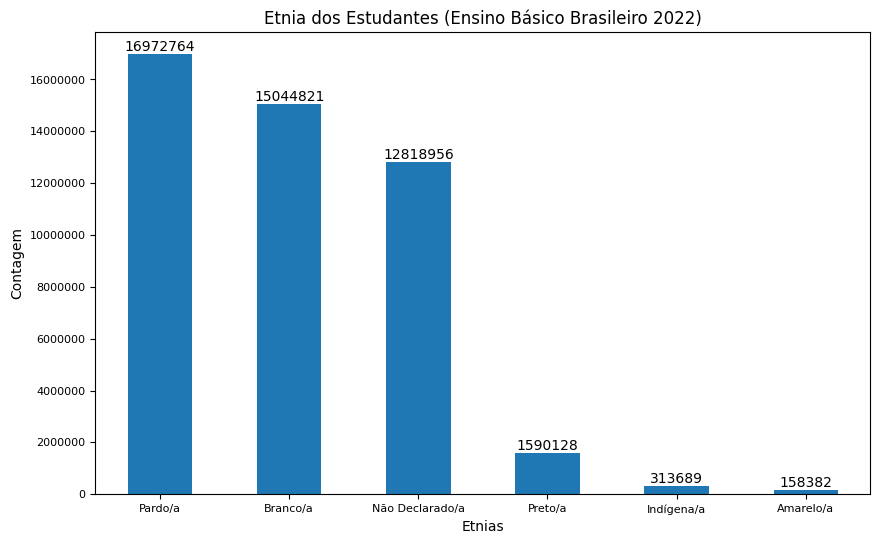
\includegraphics[width=0.8\textwidth]{Textuais/Imagens/Gráficos/etnia_brasil.png}
    \label{fig:etnia-brasil}
    \fonte{\me{2023}}
\end{figure}


A dependência administrativa das escolas pode exercer uma influência na permanência do estudante, escolas municipais e estaduais, muitas vezes, diferem em termos de recursos financeiros, infraestrutura, qualidade do ensino e programas pedagógicos, o que pode afetar diretamente a taxa de evasão escolar. Portanto, a dependência administrativa é apenas um dos muitos fatores que podem influenciar a permanência do estudante na escola. O gráfico da Figura \ref{fig:dependecia} é um gráfico de pizza que ilustra a ``Dependência Administrativa das Escolas'', que destaca a divisão entre escolas municipais e estaduais no contexto geral da pesquisa. Do total, uma maior porção, exatamente 62,3\%, representa as escolas municipais, enquanto as escolas estaduais compõem os restantes 37,7\%. A predominância das escolas municipais pode sugerir uma maior participação ou prevalência destas na amostra de estudantes que responderam ao questionário. Para ter um melhor comparativo entre os estados, a Tabela \ref{tab:dep_adm_escolas_estado} mostra a divisão entre os estados, notando-se uma forte representatividade das escolas municipais na maioria dos estados, com exceção de Goías, Minas Gerais, Roraima, São Paulo e Tocantins.



% Escolas municipais, geridas pelos governos locais, podem ter melhor capacidade de atender às necessidades específicas da sua comunidade imediata. Elas podem oferecer programas que são mais alinhados com o contexto local e, com a proximidade administrativa, podem ser mais receptivas às sugestões e necessidades dos estudantes e pais. Contudo, dependendo do município, essas escolas podem sofrer com a falta de recursos, o que pode levar à infraestrutura precária e à falta de materiais didáticos e professores qualificados, contribuindo para a evasão escolar.

% Por outro lado, as escolas estaduais, gerenciadas pelos governos estaduais, podem ter acesso a um orçamento maior e a uma estrutura administrativa mais ampla. Isso pode resultar em melhor infraestrutura e recursos, programas de formação continuada para professores e projetos educacionais de maior alcance. No entanto, a gestão centralizada pode não ser tão sensível às necessidades locais e, às vezes, pode resultar em políticas genéricas que não atendem às particularidades de cada comunidade.

% Além disso, a formação e a retenção de professores podem variar substancialmente entre as escolas municipais e estaduais, influenciando a qualidade do ensino e, consequentemente, a permanência dos alunos. Professores mais qualificados e bem remunerados podem ser mais prevalentes em escolas estaduais, resultando em melhores resultados educacionais e menor evasão.

% Por fim, a evasão escolar pode ser impactada pela governança e pelas políticas educacionais em vigor em cada nível administrativo. Programas de intervenção focados na redução da evasão escolar, como o acompanhamento individualizado de estudantes em risco, investimentos em aconselhamento e apoio psicológico, bem como a implementação de métodos pedagógicos inovadores, podem ser adotados de maneira diferente pelas escolas municipais e estaduais.



\begin{figure}[ht!]
    \centering
    \caption{Taxa de porcentagens das dependências administrativas das escolas}
    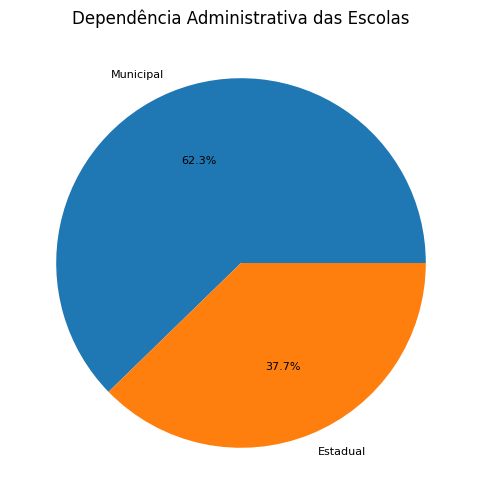
\includegraphics[width=0.5\textwidth]{Textuais/Imagens/Gráficos/dependenciaadm.png}
    \label{fig:dependecia}
    \fonte{\me{2023}}
\end{figure}

\begin{table}[ht!]
\centering
\caption{Dependência administrativa das escolas dividida por estado}
\label{tab:dep_adm_escolas_estado}
\resizebox{\textwidth}{!}{%
\begin{tabular}{|c|c|c|c|c|c|c|c|c|c|c|c|c|c|c|c|c|c|c|c|c|c|}
\hline
\textbf{UF}        & AL & AM & BA & CE & DF & ES & GO & MA & MG & MS & PA & PB & PE & PI & RJ & RN & RR & SC & SE & SP & TO \\ \hline
\textbf{Estadual}  & 0  & 1  & 0  & 0  & 1  & 0  & 29 & 0  & 13 & 1  & 16 & 0  & 0  & 0  & 0  & 0  & 4  & 0  & 2  & 5  & 27 \\ \hline
\textbf{Municipal} & 7  & 1  & 26 & 19 & 0  & 1  & 0  & 21 & 1  & 1  & 85 & 4  & 2  & 16 & 2  & 8  & 0  & 1  & 3  & 0  & 11 \\ \hline
\end{tabular}%
}
\fonte{\me{2023}}
\end{table}



%%%%%%%%%%%%%%%%%%%%%%%%%%%%%%%%%%%%%%
%%%%%%%%%%%%%%%%%%%%%%%%%%%%%%%%%%%%%%
%%%%%%%%%%%%%%%%%%%%%%%%%%%%%%%%%%%%%%
%%%%%%%%%%%%%%%%%%%%%%%%%%%%%%%%%%%%%%


%%%%%%%%%%%%%%%%%%%%%%%%%%%%%%%%%%%%%%